En este capítulo se presenta las simulaciones realizadas para verificar el correcto funcionamiento de la
red diseñada. Se ha llevado varias simulaciones de la red utilizando GNS3, en
las cuáles se ha dividido en cuatro partes:
\begin{itemize}
	\item Simulación de la red ISP.
	\item Simulación de la Oficina Central.
	\item Simulación entre sedes remotas y red ISP.
	\item Laboratorio de pruebas.
\end{itemize}

Se han hecho diferentes simulaciones debido a las limitaciones del hardware del ordenador de realización de este proyecto, por lo que impide simular la red completa en una sola simulación.

\section{Simulación de la red de ISP}
\label{sec:simulacion_red_isp}
Para la simulación de la red ISP se va basar en MPLS VPN L3, aunque en el diseño de la red final se ha optado SD-WAN con Cisco Meraki para la interconexión de las distintas sedes, esta decisión se ha tomado por las limitaciones técnicas de GNS3 el cual no permite emular estos dispositivos, ya que ésta solución depende de una infraestructura en la nube gestionada directamente por ellos. Además, muchas de las funcionalidades clave que definen a una solución SD-WAN, como la gestión centralizada, la aplicación de políticas dinámicas por el tipo de tráfico y el monitoreo inteligente de enlaces, estan fuera del alcance de GNS3. Replicar este entorno de forma precisa en este simulador de redes es complejo, poco escalable y alejadas al funcionamiento real de Meraki, perdiendo así la esencia de esta tecnología que es la simplicidad operativa, la visibilidad completa de la red y el control centralizado del tráfico.

\vspace{0.5cm}
Por otro lado, si bien existen imágenes de soluciones SD-WAN que pueden encontrarse en entornos de pruebas, estas requieren licencias oficiales para poder ser utilizadas, lo que representa una limitación importante.

\vspace{0.5cm}
Es por ello que se ha optado por simular una red MPLS VPN L3, que es una tecnología ampliamente utilizada para la interconexión de sedes a través de un \textit{backbone} común y la gestión de tráfico entre ellas. Esta tecnología permite crear redes privadas virtuales (RPV) que proporciona conectividad segura y eficiente entre las distintas sedes, permitiendo el transporte de datos a través de un único canal troncal compartido.

\vspace{0.5cm}
De esta forma, se han usado los routers \texttt{MikroTik CHR 7.16} \cite{mikrotik_cloud_hosted_router} que son dispositivos virtuales que permiten simular el comportamiento de un router físico. Estos dispositivos son ideales para la simulación de la red MPLS, ya que ofrecen una amplia gama de funcionalidades y son compatibles con los
protocolos utilizados en la red. El único inconveniente es que RouterOS, el sistema operativo de MikroTik, no es compatible con IPv6 para MPLS, por lo que se ha optado por utilizar IPv4 para la simulación.

\vspace{0.5cm}
Se ha utilizado el rango de direcciones privadas 10.0.0.0/30 y 172.16.0.0/30 para los enlaces punto a punto entre routers empleando subredes /30. Además, se han asignado direcciones /32 del rango 1.1.1.0/32 a las interfaces loopback de cada router. Esta estructura permite una separación lógica y ordenada entre los distintos tipos de tráfico en la red MPLS, diferenciando claramente el tráfico interno de cada sede del tráfico troncal entre sedes.

\vspace{0.5cm}
La asignación de direcciones /32 a las interfaces loopback permite identificar de forma única a cada router dentro del dominio MPLS, facilitando la operación de protocolos como LDP y BGP. Incluso en el caso de ciertos routers que no
pertenecen directamente a la red MPLS, como los CE, se utilizan estas direcciones para mantener una identificación coherente dentro del diseño general. Por otro lado, las subredes /30 se emplean en los enlaces punto a punto para asegurar una utilización eficiente del espacio de direcciones IP, reduciendo el desperdicio.

\vspace{0.5cm}
En la Figura~\ref{fig:red_mpls} se muestra la red MPLS configurada en GNS3, que incluye los routers PE (Provider Edge) que son los encargados de conectar las sedes a la red MPLS, P (Provider) que son responsables de enrutar el tráfico entre las distintas sedes y los CE (Customer Edge) que son los encargados de conectar la red local a la red MPLS.

\begin{figure}[H]
	\centering
	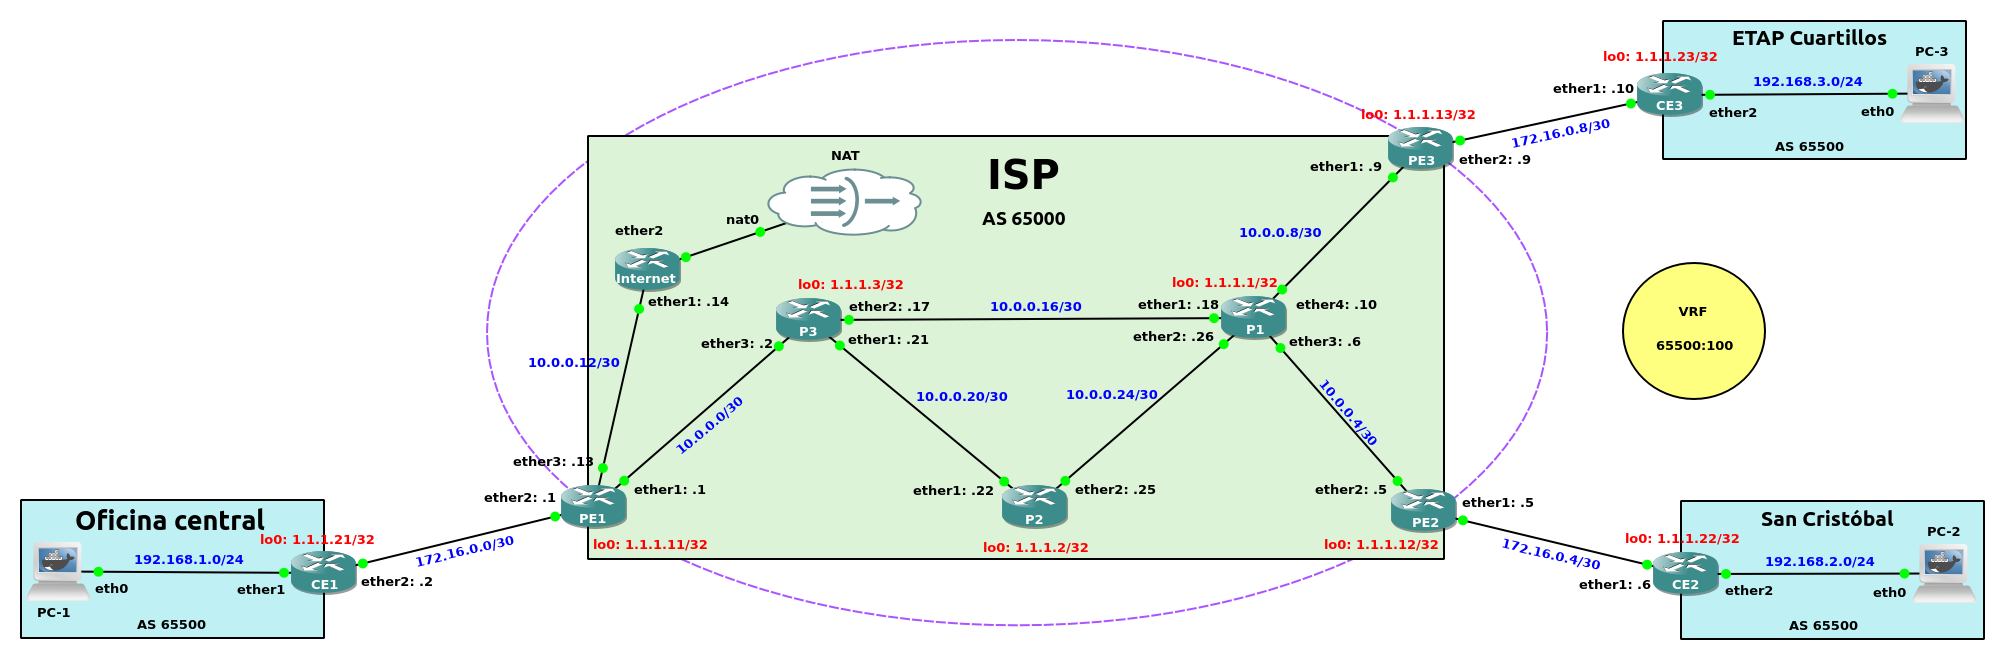
\includegraphics[width=1\textwidth]{images/red_mpls.png}
	\caption{Red MPLS configurada en GNS3}
	\label{fig:red_mpls}
\end{figure}

\newpage

\noindent
A continuación, en la Tabla~\ref{tab:esquema_direccionamiento_isp} se muestra el esquema de direccionamiento implementado en la red MPLS:
\begin{table}[H]
	\centering
	\begin{subtable}[b]{0.475\textwidth}
		\centering
		\begin{tabular}{|l|l|l|}
			\hline
			\textbf{Router} & \textbf{Interfaz} & \textbf{Dirección IP} \\ \hline
			PE1             & Lo0               & 1.1.1.11/32           \\ \cline{2-3}
			                & ether1            & 10.0.0.1/30           \\ \cline{2-3}
			                & ether2            & 172.16.0.1/30         \\ \cline{2-3}
			                & ether3            & 10.0.0.14/30          \\ \hline
			PE2             & Lo0               & 1.1.1.12/32           \\ \cline{2-3}
			                & ether1            & 172.16.0.5/30         \\ \cline{2-3}
			                & ether2            & 10.0.0.5/30           \\ \hline
			PE3             & Lo0               & 1.1.1.13/32           \\ \cline{2-3}
			                & ether1            & 10.0.0.9/30           \\ \cline{2-3}
			                & ether2            & 172.16.0.9/30         \\ \hline
			P1              & Lo0               & 1.1.1.1/32            \\ \cline{2-3}
			                & ether1            & 10.0.0.18/30          \\ \cline{2-3}
			                & ether2            & 10.0.0.26/30          \\ \cline{2-3}
			                & ether3            & 10.0.0.6/30           \\ \cline{2-3}
			                & ether4            & 10.0.0.10/30          \\ \hline
			P2              & Lo0               & 1.1.1.2/32            \\ \cline{2-3}
			                & ether1            & 10.0.0.22/30          \\ \cline{2-3}
			                & ether2            & 10.0.0.25/30          \\ \hline
		\end{tabular}
	\end{subtable}
	\hfill
	\begin{subtable}[b]{0.475\textwidth}
		\centering
		\begin{tabular}{|l|l|l|}
			\hline
			\textbf{Router} & \textbf{Interfaz} & \textbf{Dirección IP} \\ \hline
			P3              & Lo0               & 1.1.1.3/32            \\ \cline{2-3}
			                & ether1            & 10.0.0.21/30          \\ \cline{2-3}
			                & ether2            & 10.0.0.17/30          \\ \cline{2-3}
			                & ether3            & 10.0.0.2/30           \\ \hline
			CE1             & Lo0               & 1.1.1.21/32           \\ \cline{2-3}
			                & ether1            & 192.168.1.1/24        \\ \cline{2-3}
			                & ether2            & 172.16.0.2/30         \\ \hline
			CE2             & Lo0               & 1.1.1.22/32           \\ \cline{2-3}
			                & ether1            & 192.168.2.1/24        \\ \cline{2-3}
			                & ether2            & 172.16.0.6/30         \\ \hline
			CE3             & Lo0               & 1.1.1.23/32           \\ \cline{2-3}
			                & ether1            & 192.168.3.1/24        \\ \cline{2-3}
			                & ether2            & 172.16.0.10/30        \\ \hline
			Internet        & Lo0               & 1.1.1.14/32           \\ \cline{2-3}
			                & ether1            & 10.0.0.14/30          \\ \cline{2-3}
			                & ether2            & DHCP                  \\ \hline
		\end{tabular}
	\end{subtable}
	\caption{Esquema de direccionamiento para la red ISP}
	\label{tab:esquema_direccionamiento_isp}
\end{table}

Este esquema permite una gestión eficiente del tráfico entre las sedes,
garantizando la conectividad y la seguridad de los datos que circulan por la
red MPLS. Las direcciones IP asignadas a cada dispositivo son únicas dentro de
la red MPLS, lo que facilita la identificación y el enrutamiento de los
paquetes de datos.

\subsection{Configuración de interfaces loopback y asignar IPs a interfaces físicas}
En el contexto de una red MPLS, es imprescindible establecer una única sesión
LDP (Label Distribution Protocol) entre cada par de routers con el fin de
permitir el correcto intercambio de etiquetas. Para garantizar que este proceso
no se vea afectado por el estado operativo o el direccionamiento de las
interfaces físicas utilizadas para el reenvío de tráfico, se recurre
habitualmente al uso de interfaces loopback. Estas proporcionan una dirección
IP estable y siempre activa, independientemente de las condiciones de los
enlaces físicos.

\vspace{0.5cm}
En consecuencia, es necesario configurar una interfaz
loopback en cada uno de los routers que integran la infraestructura MPLS. Para
ello, se implementará una interfaz de tipo \textit{bridge} sin asociación a puertos
físicos, a la cual se asignará una dirección IP o subred previamente reservada
para las sesiones LDP dentro de la red. Esta configuración contribuye a una
mayor estabilidad y resiliencia en el establecimiento de las rutas MPLS.

\newpage

\vspace{0.5cm}
A continuación, se presenta un ejemplo de configuración de una interfaz
loopback en un router MikroTik:

\begin{lstlisting}[language=RouterOS]
[admin@MikroTik] > /system identity set name=PE1
[admin@PE2] > /interface bridge add name=lo0
[admin@PE2] > /ip address add address=1.1.1.12/32 interface=lo0
\end{lstlisting}

En cuanto a la configuración de las interfaces físicas, se han asignado
direcciones IP a las interfaces de los routers que se conectan entre sí. Por
ejemplo, en el router PE2 se ha configurado de la siguiente manera:

\begin{lstlisting}[language=RouterOS]
[admin@PE2] > /ip address add address=172.16.0.5/30 interface=ether1
[admin@PE2] > /ip address add address=10.0.0.5/30 interface=ether2
\end{lstlisting}

\subsection{OSPF como protocolo de enrutamiento}
Empezaremos aplicando el protocolo OSPF para aprender de forma dinámica las
direcciones de los routers que pertenecen a MPLS, es decir, los routers PE y P.
Por tanto, las interfaces que no pertenecen a la red MPLS no se incluirán en el
proceso de aprendizaje.

\vspace{0.5cm}  Para ello, se ha creado una instancia OSPF y se
han añadido las redes correspondientes a la misma. A continuación, se muestra
un ejemplo de configuración de OSPF en el router P1:
\begin{lstlisting}[language=RouterOS]
[admin@P1] > /routing ospf instance set redistribute-connected=as-type-1 numbers=0
[admin@P1] > /routing ospf network add area=backbone network=10.0.0.16/30 
[admin@P1] > /routing ospf network add area=backbone network=10.0.0.24/30 
[admin@P1] > /routing ospf network add area=backbone network=10.0.0.4/30 
[admin@P1] > /routing ospf network add area=backbone network=10.0.0.8/30 
\end{lstlisting}

%
% Se deberá aplicar una configuración equivalente en todos los enrutadores de la
% red MPLS, una vez hecho, por ejemplo, en P1 obtendremos la siguiente tabla de
% enrutamiento:
En la Figura~\ref{fig:routing_table} se muestra la tabla de enrutamiento del router P1, que refleja las rutas aprendidas a través del protocolo OSPF.

\begin{figure}[H]
	\centering
	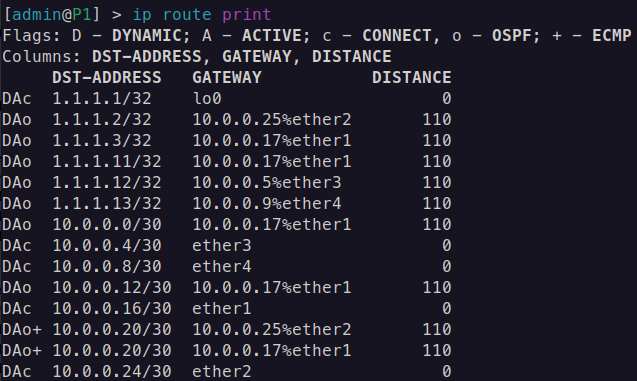
\includegraphics[width=0.8\textwidth]{images/routing_table.png}
	\caption{Tabla de enrutamiento de P1}
	\label{fig:routing_table}
\end{figure}

\subsection{Configuración de la distribución de etiquetas (LDP)}
Para asegurar la correcta distribución de las etiquetas MPLS asociadas a cada una
de las rutas activas en la red, es fundamental habilitar el Protocolo de Distribución de Etiquetas (LDP)
en todos los enrutadores que forman parte de la red MPLS. A continuación,
aplicaremos LDP sobre estos mismos routers, excluyendo las interfaces que se comunican
con routers externos a la backbone, ya que no requieren esta configuración. Esta configuración se
ha aplicado a todos los routers de la red MPLS, por ejemplo, en P1 se ha configurado de la siguiente manera:

\begin{lstlisting}[language=RouterOS]
[admin@P1] > /mpls ldp add afi=ip lsr-id=1.1.1.1 transport-addresses=1.1.1.1
[admin@P1] > /mpls ldp interface add interface=ether1
[admin@P1] > /mpls ldp interface add interface=ether2
[admin@P1] > /mpls ldp interface add interface=ether3
[admin@P1] > /mpls ldp interface add interface=ether4
\end{lstlisting}

Además, se ha configurado el rango de etiquetas dinámicas para el tráfico MPLS según la Tabla~\ref{tab:rango_etiquetas_mpls}.

\begin{table}[H]
	\centering
	\begin{tabular}{|l|l|l|}
		\hline
		\textbf{Router} & \textbf{Loopback} & \textbf{Rango de etiquetas} \\ \hline
		PE1             & 1.1.1.11          & 10000-11999                 \\ \hline
		PE2             & 1.1.1.12          & 12000-13999                 \\ \hline
		PE3             & 1.1.1.13          & 14000-15999                 \\ \hline
		P1              & 1.1.1.1           & 20000-21999                 \\ \hline
		P2              & 1.1.1.2           & 22000-23999                 \\ \hline
		P3              & 1.1.1.3           & 24000-25999                 \\ \hline
	\end{tabular}%
	\caption{Rango de etiquetas para cada router}
	\label{tab:rango_etiquetas_mpls}
\end{table}

\noindent
Para configurar el rango de etiquetas dinámicas, se ha utilizado el siguiente comando:
\begin{lstlisting}[language=RouterOS]
[admin@P1] > /mpls settings set dynamic-label-range=20000-21999
\end{lstlisting}

%
% Se repetirá el mismo proceso para los routers PE y P.

Para comprobar que la configuración es correcta, se ha realizado un \texttt{traceroute} desde el router PE1 a PE2 y
se tendrá que ver la asignación de una etiqueta.
\begin{figure}[H]
	\centering
	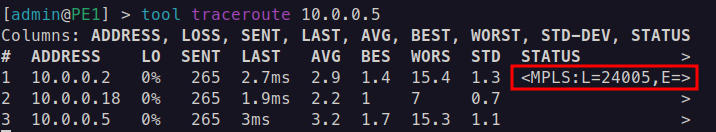
\includegraphics[width=0.8\textwidth]{images/ldp_test.png}
	\caption{Traceroute desde PE1 a PE2}
	\label{fig:traceroute}
\end{figure}

\subsection{Multi-Protocolo BGP (MP-BGP)}
El Multi-Protocolo BGP (MP-BGP) es una extensión del protocolo BGP (Border Gateway Protocol) que permite propagar direcciones y los atributos que la acompañan a través de múltiples protocolos de red. En este contexto, los Sistemas Autónomos (AS) representan agrupaciones de redes bajo una misma política de enrutamiento, lo que facilita la gestión y el intercambio de rutas entre diferentes dominios administrativos. Por tanto, para establecer la conectividad entre los routers PE de la red MPLS, se creará una sesión BGP entre ellos. Para ello, primero se actualizará la plantilla \texttt{default} de BGP en los routers, acorde al sistema autónomo (65000 en este caso) y al conjunto de direcciones que enrutará cada router PE.

\vspace{0.5cm}
\noindent
A continuación, se muestra un ejemplo de configuración de BGP en el router PE2:
\begin{lstlisting}[language=RouterOS]
[admin@PE2] > /routing bgp template set default address-families=ip,vpnv4 as=65000 router-id=1.1.1.12
\end{lstlisting}

Ahora, se crearán las conexiones BGP entre los otros routers PE de la red MPLS. Unicamente hay que configurar la dirección local, la dirección remota, el AS remoto, el role local de BGP (ibgp en este caso al ser routers de la misma AS) y habilitar la escucha como la conexión.
\begin{lstlisting}[language=RouterOS]
[admin@PE2] > /routing bgp connection add name=toPE1 template=default local.address=1.1.1.12 local.role=ibgp remote.address=1.1.1.11 remote.as=65000 connect=yes listen=yes
[admin@PE2] > /routing bgp connection add name=toPE3 template=default local.address=1.1.1.12 local.role=ibgp remote.address=1.1.1.13 remote.as=65000 connect=yes listen=yes
[admin@PE2] > /routing bgp connection add name=toPE4 template=default local.address=1.1.1.12 local.role=ibgp remote.address=1.1.1.14 remote.as=65000 connect=yes listen=yes
\end{lstlisting}

Una vez hecho, se podrá comprobar que se ha establecido la sesión BGP ejecutando el comando \lstinline[language=RouterOS]|/routing bgp session print| en los routers PE:

\begin{figure}[H]
	\centering
	\begin{subfigure}[b]{0.475\textwidth}
		\centering
		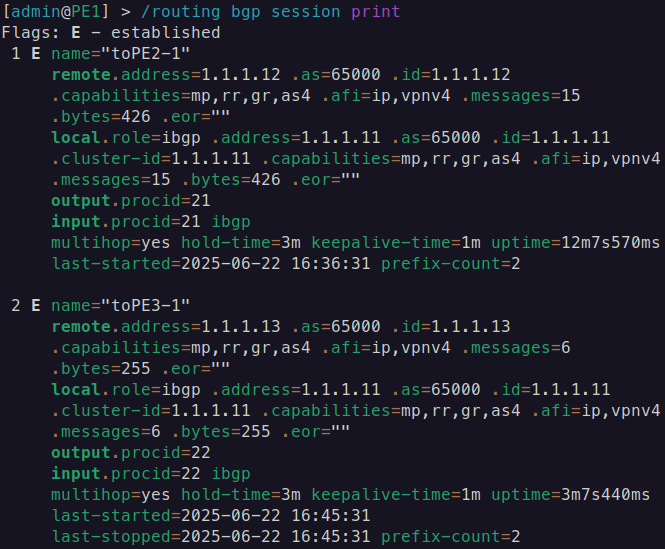
\includegraphics[width=\textwidth]{images/PE1_bgp_print.png}
		\caption{Sesiones BGP establecidas en PE1}
		\label{fig:PE1_bgp_print}
	\end{subfigure}
	\hfill
	\begin{subfigure}[b]{0.482\textwidth}
		\centering
		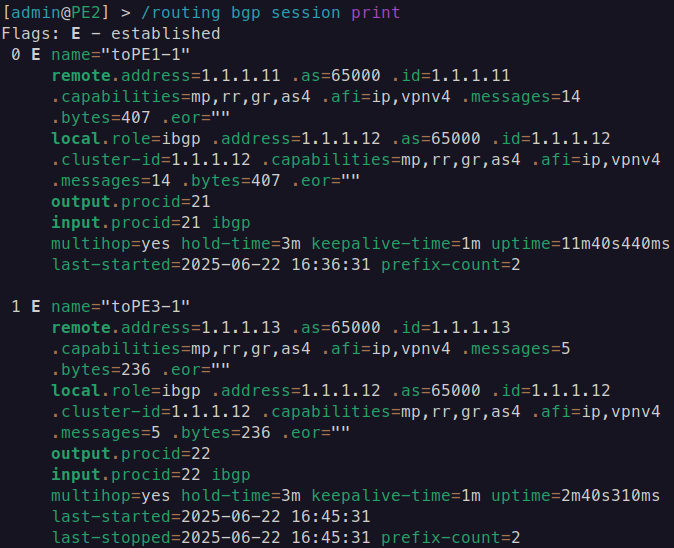
\includegraphics[width=\textwidth]{images/PE2_bgp_print.png}
		\caption{Sesiones BGP establecidas en PE2}
		\label{fig:PE2_bgp_print}
	\end{subfigure}
	\caption{Sesiones BGP establecidas en PE1 y PE2}
	\label{fig:PE1_PE2_PE3_bgp_print}
\end{figure}

\subsection{Configuración de VRF y VPN}
Virtual Routing and Forwarding (VRF) es una tecnología que permite que múltiples
instancias de una tabla de enrutamiento coexistan en el mismo router. Las sedes se
situarán en una tabla VRF configurada con un RD (Route Distinguisher) y un RT (Route Target)
de importación y exportación. El RD es un identificador de rutas VPN que se antepone a la dirección
de red para formar un prefijo único (ASN:número de ruta). El RT es el valor numérico definido por
cada PE que está asociado a las rutas que exporta a los puertos BGP. Existen dos tipos de RT:

\begin{itemize}
	\item \textbf{RT de exportación:} Identifican los sitios remotos a los que se exportan las rutas.
	\item \textbf{RT de importación:} Utilizados por los routers PE para importar las rutas en sus tablas VRF.
\end{itemize}

Para la configuración, antes se crearán las VRFs unicamente en los routers PE que servirán para consultar el direccionamiento de las sedes que están conectadas a la red MPLS. Se creará una tabla VRF por router PE de la siguiente manera:
\begin{lstlisting}[language=RouterOS]
[admin@PE2] > /ip vrf add name=CE2 interfaces=ether1 
\end{lstlisting}

Ahora, se configurará la VPN a través de BGP en los routers PE. Se definirá el \texttt{Router Distinguishers (RD)}, el cual identifica la ruta VPN y es representado como ASN:número de ruta.

\vspace{0.5cm}
También se definirán los \texttt{Route Target (RT)} de exportación y de importación, que indicarán qué rutas se distribuirán al peer PE según la VPN que identifique. En este caso, se ha definido el mismo valor para RD y RT.

\vspace{0.5cm}
Finalmente, se especificará la política de asignación de etiquetas, la tabla VRF que se empleará y el tipo de rutas que se compartirán desde la VRF hacia VPNv4. Además de las rutas estáticas (static) y conectadas (connected), se activará BGP, dado que este será el protocolo utilizado entre los routers PE y CE en su variante External BGP (eBGP).

\begin{lstlisting}[language=RouterOS]
[admin@PE2] > /routing bgp vpn add route-distinguisher=65000:100 import.route-targets=65000:100 vrf=CE2 label-allocation-policy=per-vrf export.route-targets=65000:100 .redistribute=connected,static,bgp
\end{lstlisting}

\subsection{Comunicación entre routers PE y CE}
Para garantizar la conectividad entre los routers PE y CE, implementaremos el protocolo eBGP, asignando un número de sistema autónomo (AS) distinto al de la red troncal MPLS, específicamente el AS 65500.

\subsubsection*{Configuración de los routers PE}
En los routers PE, se van a crear nuevas conexiones BGP con los routers CE. Se va a indicar la dirección local, el AS local, el role local, el AS remoto, la dirección remota, y a habilitar la conexión y la escucha. Además, hay que indicar el ID del router que será la interfaz loopback, el \texttt{VRF} que se usará y la tabla de routing asociada al \texttt{VRF}. Por último, para asegurar que todas las rutas puedan ser anunciadas por la red MPLS, es necesario configurar \texttt{output.default-originate=always}. Esta acción genera una ruta por defecto en el router CE, la cual se aprende mediante eBGP y es crucial para la comunicación de direcciones privadas a través de MPLS.

\begin{lstlisting}[language=RouterOS]
[admin@PE2] > /routing bgp connection add name=toCE2 router-id=1.1.1.12 as=65000 local.address=172.16.0.5 .role=ebgp remote.address=172.16.0.6 .as=65500 routing-table=CE2 vrf=CE2 connect=yes listen=yes output.default-originate=always
\end{lstlisting}

\subsubsection*{Configuración de los routers CE}
Para los routers CE, hay una lista de direcciones que se van a exportar a través de BGP. En esta lista de direcciones se asignarán a la conexión BGP para permitir que los paquetes recibidos en el CE puedan ser enviados a través de la red MPLS.
\begin{lstlisting}[language=RouterOS]
[admin@CE2] > /ip firewall address-list add address=192.168.2.0/24 list=BGP_OUT
\end{lstlisting}

Ahora con la lista direcciones creada, se puede configurar la conexión BGP entre el router CE y el router PE. Se indicará el ID del router, AS, dirección local, role local, dirección remota, AS remoto y la lista de direcciones que se van a exportar. También se activará la conexión y la escucha.
\begin{lstlisting}[language=RouterOS]
[admin@CE2] > /routing bgp connection add name=toPE2 as=65500 router-id=1.1.1.22 local.address=172.16.0.6 .role=ebgp remote.address=172.16.0.5 remote.as=65000 output.network=BGP_OUT connect=yes listen=yes
\end{lstlisting}

Con las conexiones BGP configuradas, se puede comprobar que se ha establecido la sesión BGP ejecutando el comando \lstinline[language=RouterOS]|/routing bgp session print| en los routers CE:

\begin{figure}[H]
	\centering
	\begin{subfigure}[b]{0.48\textwidth}
		\centering
		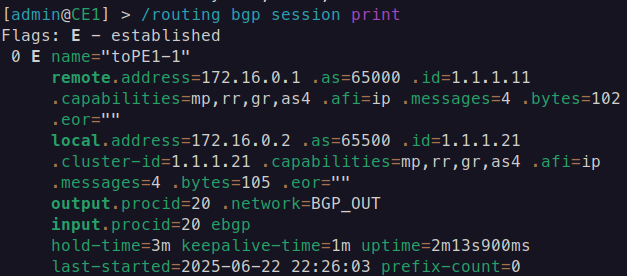
\includegraphics[width=\textwidth]{images/CE1_bgp_print.png}
		\caption{Sesiones BGP establecidas en CE1}
		\label{fig:CE1_bgp_print}
	\end{subfigure}
	\hfill
	\begin{subfigure}[b]{0.48\textwidth}
		\centering
		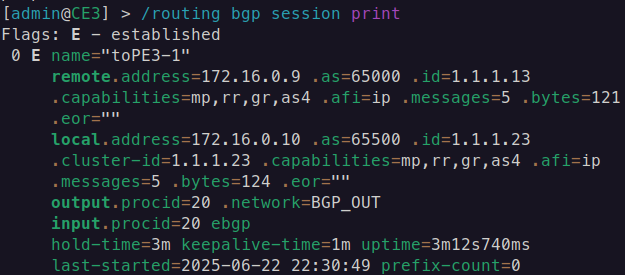
\includegraphics[width=\textwidth]{images/CE3_bgp_print.png}
		\caption{Sesiones BGP establecidas en CE3}
		\label{fig:CE3_bgp_print}
	\end{subfigure}
	\caption{Sesiones BGP establecidas en los routers CE}
	\label{fig:bgp_sessions}
\end{figure}

\begin{tcolorbox}[colback=gray!10!white, colframe=gray!70!black, title=NOTA:, size=title]
	\textit{Todas las configuraciones mostradas en los ejemplos anteriores se aplicarán de forma análoga en el resto de los routers, adaptando únicamente las direcciones IP, nombres de interfaces y parámetros específicos según corresponda a cada dispositivo.}
\end{tcolorbox}

\subsection{Acceso a Internet}
% PE1:
% /routing bgp template set default address-families=ip,vpnv4 as=65000 router-id=1.1.1.11
% /routing bgp connection
% add connect=yes disabled=no listen=yes local.address=1.1.1.11 .role=ibgp \
%     name=toPE2 remote.address=1.1.1.12 .as=65000 templates=default
% /routing bgp connection
% add connect=yes disabled=no listen=yes local.address=1.1.1.11 .role=ibgp \
%     name=toPE3 remote.address=1.1.1.13 .as=65000 templates=default
% /routing bgp connection
% add connect=yes disabled=no listen=yes local.address=1.1.1.11 .role=ibgp \
%     name=toPE4 remote.address=1.1.1.14 .as=65000 templates=default

% /ip vrf add name=CE1 interfaces=ether2 

% /routing bgp vpn
% add export.redistribute=connected,static,bgp .route-targets=65000:100 \
%     import.route-targets=65000:100 label-allocation-policy=per-vrf name=\
%     bgp-mpls-vpn-1 route-distinguisher=65000:100 vrf=CE1

% /routing bgp connection
% add as=65000 connect=yes disabled=yes listen=yes local.address=172.16.0.1 \
%     .role=ebgp name=toCE1 output.default-originate=always remote.address=\
%     172.16.0.2 .as=65500 router-id=1.1.1.11 routing-table=CE1 vrf=CE1

% /routing bgp connection add as=65000 connect=yes disabled=yes listen=yes local.address=172.16.0.1 .role=ebgp name=toCE1 output.default-originate=always remote.address=172.16.0.2 .as=65500 router-id=1.1.1.11 routing-table=CE1 vrf=CE1

% /ip firewall mangle
% add action=mark-routing chain=prerouting dst-address=!192.168.0.0/16 \
%     in-interface=ether2 new-routing-mark=main passthrough=yes
% /ip route add gateway=172.16.0.2@CE1 routing-table=CE1
% /ip route add gateway=10.0.0.14
% /ip route add dst-address=172.16.0.0/30 gateway=CE1@CE1 routing-table=main

% % CE1:
% /ip firewall address-list add address=192.168.1.0/24 list=BGP_OUT
% /ip firewall nat add action=masquerade chain=srcnat dst-address=!192.168.0.0/16 out-interface=ether2

% /ip route add gateway=172.16.0.1

% /routing bgp connection
% add as=65500 connect=yes listen=yes local.address=172.16.0.2 .role=ebgp name=\
%     toPE1 output.network=BGP_OUT remote.address=172.16.0.1 .as=65000 router-id=\
%     1.1.1.21


Para proporcionar acceso a Internet se ha centralizado en el router CE1 que este actuará como gateway, es decir todo el tráfico que quiera salir a Internet pasará por este router y luego volverá al router PE1 y de ahi a otro router que se conecta a Internet. Para ello, se ha configurado el router CE1 para que realice NAT (Network Address Translation) y permita que los dispositivos una red local accedan a Internet. Además, se ha quitado la conexión BGP entre el router PE1 y CE1, añadiendo una ruta estática en el router PE1 hacia CE1 dentro de la VRF CE1. La configuración de la conexión BGP entre el router PE1 y CE1 se ha realizado de la siguiente manera:
\begin{lstlisting}[language=RouterOS]
[admin@PE1] > /routing bgp connection
add as=65000 connect=yes disabled=yes listen=yes local.address=172.16.0.1 .role=ebgp name=toCE1 output.default-originate=always remote.address=172.16.0.2 .as=65500 router-id=1.1.1.11 routing-table=CE1 vrf=CE1
\end{lstlisting}

Para que el router CE1 pueda realizar NAT, se ha configurado una regla de NAT que permite que el tráfico que sale por la interfaz \texttt{ether2} (que es la interfaz conectada a Internet) sea traducido. La configuración de la regla de NAT se ha realizado de la siguiente manera:
\begin{lstlisting}[language=RouterOS]
[admin@CE1] > /ip firewall nat add action=masquerade chain=srcnat dst-address=!192.168.0.0/16 out-interface=ether2
\end{lstlisting}

Además, se ha configurado una ruta estática en el router CE1 para que el tráfico que sale a Internet pase por la interfaz \texttt{ether2}. La configuración de la ruta estática se ha realizado de la siguiente manera:
\begin{lstlisting}[language=RouterOS]
[admin@CE1] > /ip route add gateway=172.16.0.1
\end{lstlisting}

Para que el router CE1 pueda enviar tráfico a la red local, se ha configurado una ruta estática en el router PE1 hacia CE1 dentro de la VRF CE1. La configuración de la ruta estática se ha realizado de la siguiente manera:
\begin{lstlisting}[language=RouterOS]
[admin@PE1] > /ip route add dst-address=172.16.0.0/30 gateway=CE1@CE1 routing-table=main
[admin@PE1] > /ip route add gateway=172.16.0.2@CE1 routing-table=CE1
\end{lstlisting}

Por otro lado, para que el tráfico que sale por la interfaz \texttt{ether2} del router PE1 se enrute correctamente, se ha configurado una regla de mangle que marca el tráfico que no es de la red local (192.168.0.0/16) y lo enruta a través de la tabla de enrutamiento principal. La configuración de la regla de mangle se ha realizado de la siguiente manera:
\begin{lstlisting}[language=RouterOS]
[admin@PE1] > /ip firewall mangle add action=mark-routing chain=prerouting dst-address=!192.168.0.0/16 in-interface=ether2 new-routing-mark=main passthrough=yes
\end{lstlisting}

\subsection{Comprobación de la configuración}
Para comprobar que la configuración es correcta se hará un \texttt{ping} entre los PCs, por ejemplo, desde el PC1 a la IP 192.168.2.100. Pero antes hay que configurar la IP estática. Para ello, se edita el archivo \texttt{/etc/network/interfaces} y añadiendo la siguiente configuración:
\begin{lstlisting}[language=bash]
auto eth0
iface eth0 inet static
	address 192.168.X.100
	netmask 255.255.255.0
	gateway 192.168.X.1
\end{lstlisting}

\begin{tcolorbox}[colback=gray!10!white, colframe=gray!70!black, title=NOTA:, size=title]
	La X será según en que sede esté el PC. Por ejemplo, si el PC está en la Oficina Central, la X será 1.
\end{tcolorbox}

Una vez configurada la IP estática, se puede comprobar que la configuración es correcta como se ve en la Figura~\ref{fig:ping_test}.
\begin{figure}[H]
	\centering
	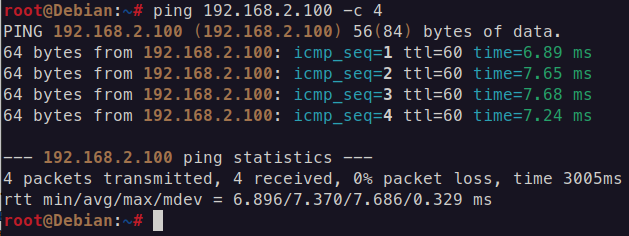
\includegraphics[width=0.75\textwidth]{images/ping_test.png}
	\caption{Comprobación de la configuración}
	\label{fig:ping_test}
\end{figure}

\section{Simulación de la Oficina Central}
La oficina central se ha configurado con un prefijo global de 2001:db8:1234:0100::/56 y
se han creado tres VLANs para segmentar el tráfico de datos, voz y DMZ. La VLAN
10 se ha asignado para el tráfico de datos, la VLAN 20 para el tráfico de voz y
la VLAN 30 para la DMZ. Por otro lado, esta sede contará con dos routers CE
(Customer Edge) configurados en alta disponibilidad mediante el protocolo VRRP
(Virtual Router Redundancy Protocol) \cite{wikipedia_vrrp}. Además, se ha configurado
un servidor DHCP para asignar direcciones IP dinámicamente a los dispositivos de la red
local y dos servidores DNS para resolver nombres de dominio y direcciones IP. La topología de switching
implementa el protocolo RSTP (Rapid Spanning Tree Protocol) \cite{wikipedia_rstp} para garantizar
redundancia en los enlaces y prevenir bucles de red, asegurando una convergencia
rápida ante fallos.
\begin{figure}[H]
	\centering
	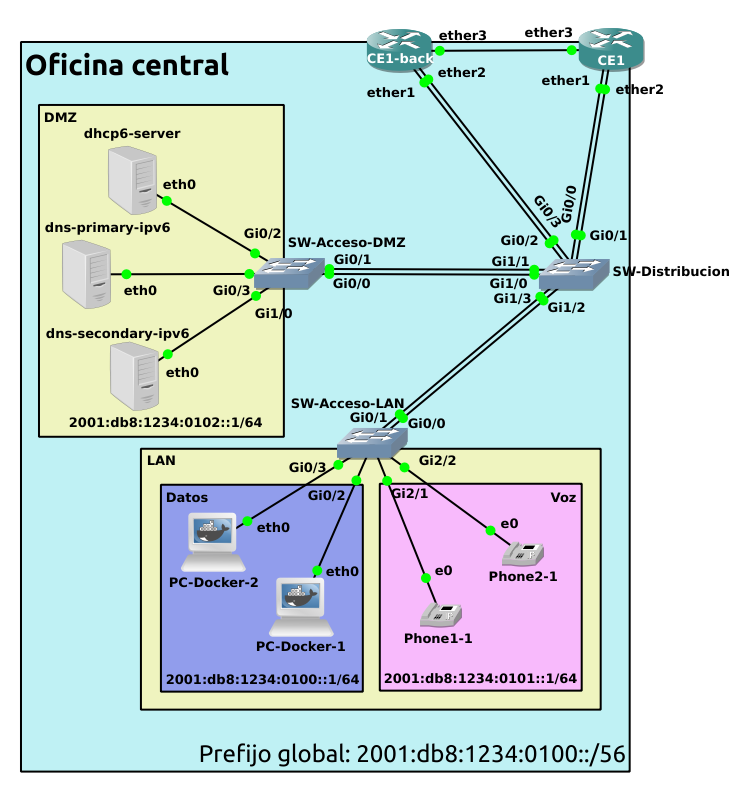
\includegraphics[width=0.8\textwidth]{images/central_office.png}
	\caption{Esquema de la oficina central}
	\label{fig:central_office}
\end{figure}

\subsection{Configuración de los routers}
Para la red local se han utilizado dos routers MikroTik CE1 \ref{Apendice2:configuracion_ce1} y CE1\_backup \ref{Apendice2:configuracion_ce1_backup} configurados con alta disponibilidad mediante VRRP y conectados a través de un enlace de sincronización dedicado. Ambos dispositivos emplean un bonding LACP (802.3ad) sobre dos interfaces físicas para mejorar la redundancia y el ancho de banda. Sobre este bonding se han definido tres VLANs: datos, voz
y DMZ, a cada una de las cuáles se le asigna una dirección IPv6. En cada VLAN se implementa VRRP, configurando CE1 como maestro (prioridad 150) y CE1\_backup como respaldo (prioridad 100), y se asignan direcciones virtuales que actúan como gateway para los dispositivos de la red. Además, se configura un relay DHCPv6 en las VLANs de datos y voz, se anuncian los servidores DNS mediante Neighbor Discovery \cite{wikipedia_nd} y se aplica un firewall básico para IPv6.

\vspace{0.5cm}
Para comprobar el funcionamiento de la configuración VRRP, se a ha ejecutado en el router CE1 el comando \lstinline[language=RouterOS]|/interface vrrp print| y se ha obtenido lo que se muestra en la Figura~\ref{fig:vrrp_output_1}.

\begin{figure}[H]
	\centering
	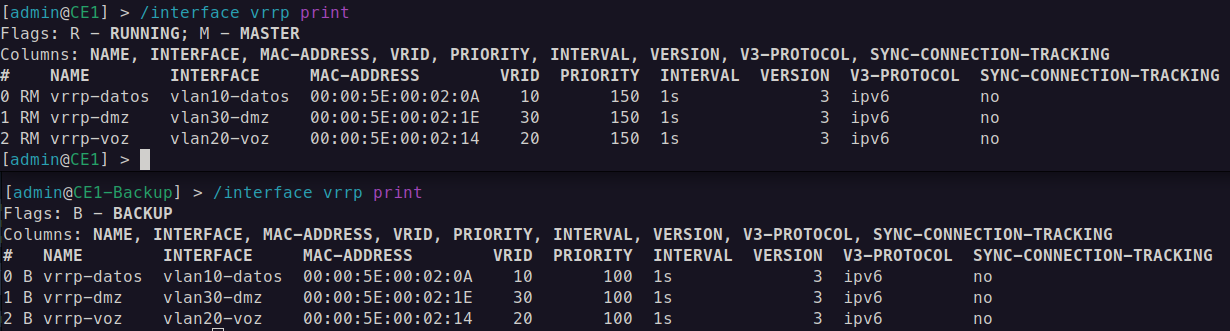
\includegraphics[width=1\textwidth]{images/vrrp_output_1.png}
	\caption{Estado de los VRRP en el router CE1}
	\label{fig:vrrp_output_1}
\end{figure}

Al ejecutar el comando, en el CE1, se puede observar que están las letras \texttt{R} y \texttt{M} que significa que están en \textit{RUNNING} y \textit{MASTER} respectivamente, confirmando que es el router maestro de VRRP. Además, se puede ver que el \texttt{Priority} es 150, es decir, que tiene más prioridad que el router CE1\_Backup que tiene el
\texttt{Priority} en 100. Otra prueba que se hizo es apagar temporalmente la interfaz VLAN 10 del router CE1 y se puede ver que el router CE1\_Backup se convierte en maestro en esta interfaz, siendo anterior el maestro. En la Figura~\ref{fig:vrrp_output_2} se puede ver el estado de los VRRP en el router CE1\_Backup.
\begin{figure}[H]
	\centering
	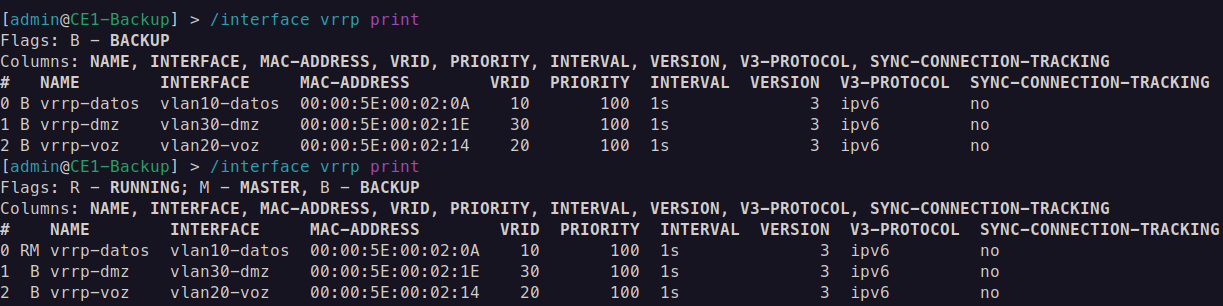
\includegraphics[width=1\textwidth]{images/vrrp_output_2.png}
	\caption{Estado de los VRRP en el router CE1\_Backup}
	\label{fig:vrrp_output_2}
\end{figure}

Otra comprobación, como se muestra en la Figura~\ref{fig:test_DHCP6_pc}, es la correcta asignación de direcciones IPv6 y conectividad con la interfaz VRRP de cada VLAN. En la izquierda
un telefono en la VLAN 20 y en la derecha un PC en la VLAN 10.

\begin{figure}[H]
	\centering
	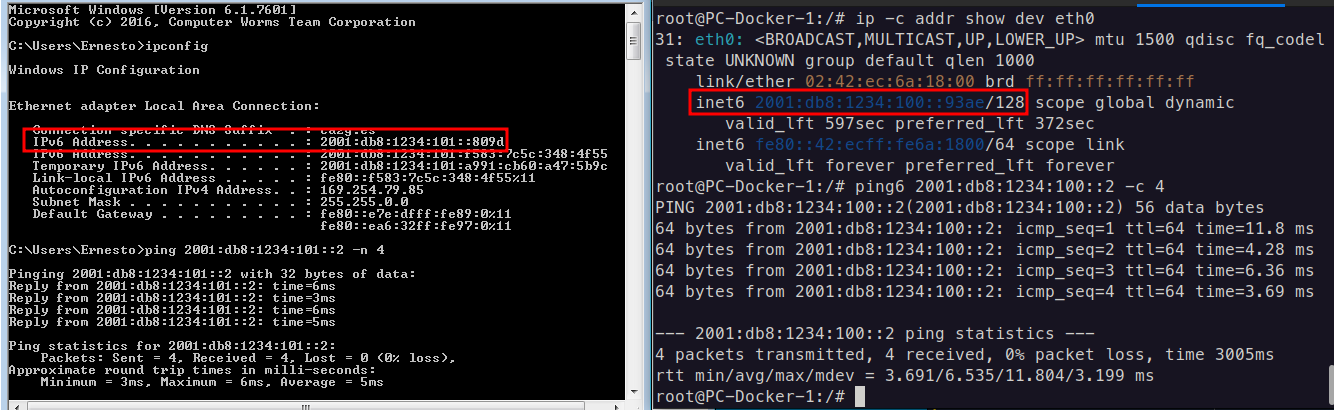
\includegraphics[width=1\textwidth]{images/test_DHCP6_ping.png}
	\caption{Asignación y conectividad IPv6}
	\label{fig:test_DHCP6_pc}
\end{figure}

Además, si desde un host se pide otra dirección IPv6, se puede ver que se obtiene una dirección ofrecida por el relay DHCPv6. En la Figura~\ref{fig:dhclient_ok} se puede ver que un host de la VLAN 10 obtiene la dirección 2001:db8:1234:100::93ae.

\begin{figure}[H]
	\centering
	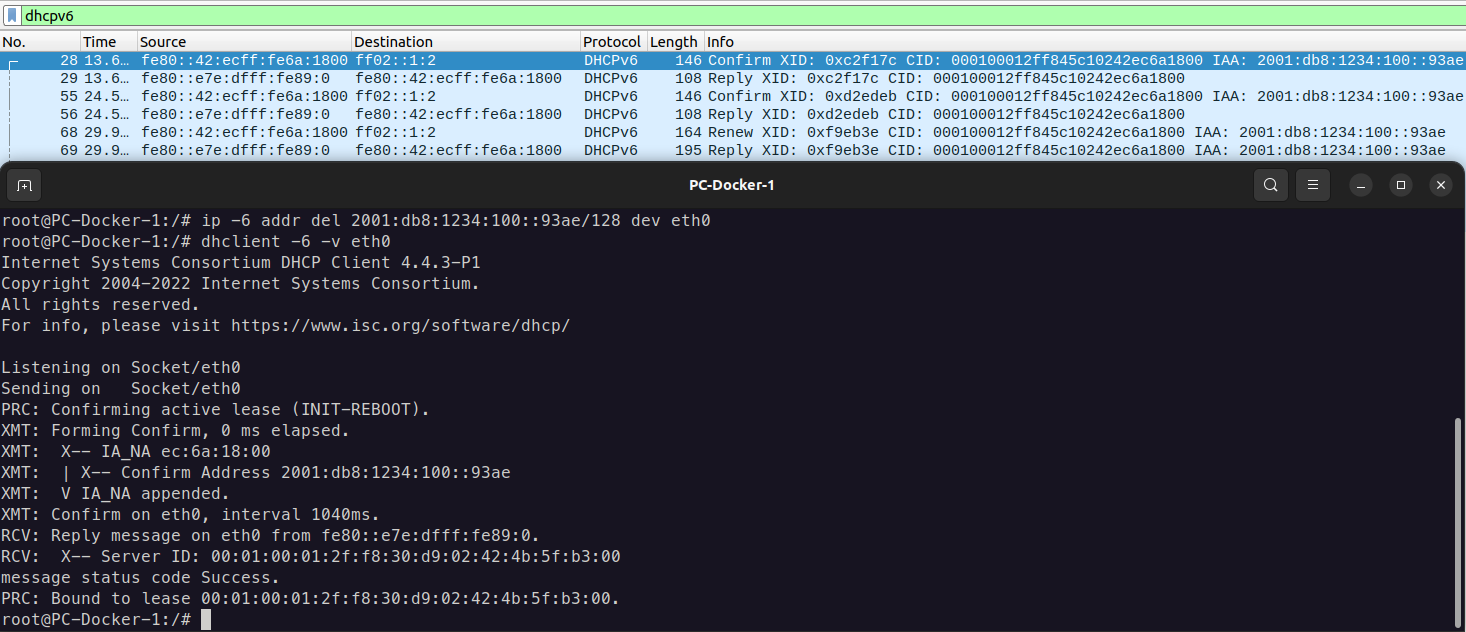
\includegraphics[width=0.95\textwidth]{images/dhclient_ok.png}
	\caption{Obtención de una dirección IPv6}
	\label{fig:dhclient_ok}
\end{figure}

% \begin{itemize}
%     \item Comprobación de la correcta asignación de direcciones IPv6 y conectividad entre hosts de cada VLAN.
%     \item Verificación del funcionamiento del failover de VRRP: ante la caída del router maestro (CE1), el router de respaldo (CE1\_backup) asume el rol de maestro sin pérdida de conectividad.
%     \item Prueba del relay DHCPv6: los hosts de las VLANs de datos y voz obtienen direcciones IPv6 dinámicas correctamente.
%     \item Comprobación de la recepción de los servidores DNS mediante Neighbor Discovery (RA).
%     \item Prueba de la comunicación entre ambos routers a través del enlace de sincronización dedicado.
% \end{itemize}

\subsection{Configuración de los switches}
En la simulación se han utilizado tres switches: uno de distribución \ref{Apendice2:configuracion_switch_distribucion_central} y dos de acceso. El switch de distribución se encarga de conectar los switches de acceso, uno a la red local \ref{Apendice2:configuracion_switch_acceso_lan_central} y otro a la DMZ \ref{Apendice2:configuracion_switch_acceso_dmz_central}. Los switches de acceso conectan los dispositivos finales a la red.

\vspace{0.5cm}
Se han configurado las VLANs en los switches para segmentar el tráfico de datos, voz y DMZ. Además, se ha implementado el protocolo Rapid Spanning Tree Protocol (RSTP), que permite una convergencia más rápida ante fallos de enlace en comparación con el STP tradicional.

\vspace{0.5cm}
Por otra parte, para aprovechar los enlaces redundantes entre los switches y aumentar el rendimiento de la red, se ha implementado EtherChannel utilizando el protocolo LACP (Link Aggregation Control Protocol). Esto permite agrupar múltiples enlaces físicos en un único enlace lógico, lo cual proporciona redundancia y balanceo de carga sin que los puertos se bloqueen por RSTP.

\vspace{0.5cm}
Para verificar el funcionamiento de RSTP, se ha utilizado el comando \lstinline[language=CiscoIOS]|show spanning-tree| en los switches, que muestra el estado de las VLANs y sus interfaces asociadas. Como ejemplo, desde el switch de acceso a la LAN, al ejecutar el comando
\lstinline[language=CiscoIOS]|show spanning-tree vlan 10|, se obtiene lo que se muestra en la Figura~\ref{fig:spanning_tree_vlan10}, donde se puede ver que el protocolo RSTP está habilitado y funcionando adecuadamente, y que el Root Bridge de la VLAN 10 es el switch de distribución. También, el enlace hacia el Root Bridge se establece a través
de la interfaz Port-channel4, correspondiente a un EtherChannel configurado con LACP, que se encuentra en estado Root Forwarding. Esto indica que el enlace lógico está activo y es utilizado como camino principal hacia el Root Bridge, sin necesidad de bloquear enlaces físicos. Luego, los demás puertos del switch aparecen en estado Designated Forwarding, lo que demuestra que están activos y conectan con los dispositivos finales. El hecho de que no existan puertos en estado de bloqueo confirma que EtherChannel está funcionando, evitando bucles sin que RSTP tenga que bloquear enlaces individuales.

\begin{figure}[htb]
	\centering
	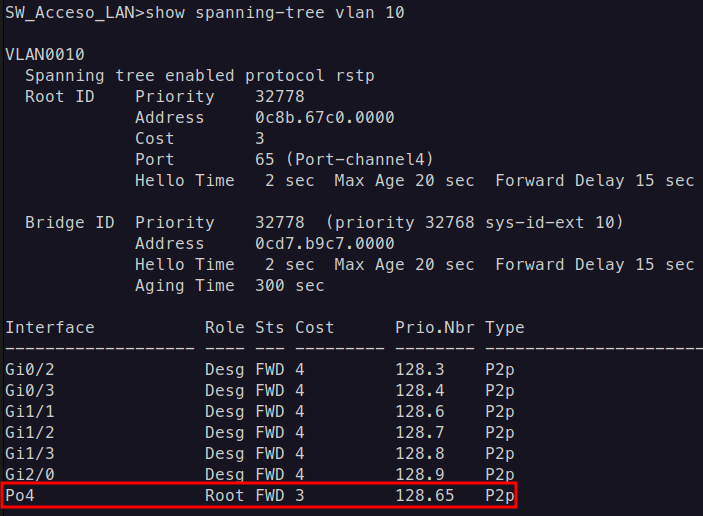
\includegraphics[width=0.7\textwidth]{images/testSTP_SWLAN2SWDistribucion_Central.png}
	\caption{Estado del protocolo Spanning Tree}
	\label{fig:spanning_tree_vlan10}
\end{figure}

\subsection{Configuración del servidor DHCP}
Para el servidor DHCP, se ha utilizado \texttt{isc-dhcp-server} sobre un contenedor Docker basado en Ubuntu 20.04, con una configuración automatizada mediante un Dockerfile \ref{Apendice2:dockerfile_dhcp}. El servidor se ha configurado con una IP estática 2001:db8:1234:0102::132/64 y se han definido rangos de direcciones IP para cada segmento de red, asegurando que los dispositivos conectados reciban direcciones válidas según el segmento al que pertenezcan. El archivo de configuración principal se encuentra en \texttt{/etc/dhcp/dhcpd6.conf} \ref{Apendice2:dhcpd6.conf}, donde se especifican los tiempos de concesión, las opciones de dominio y servidores DNS, así como las subredes correspondientes. Para las VLANs se han definido los siguientes rangos de direcciones IPv6:
\begin{itemize}
	\item \textbf{Red de datos:} rango \texttt{2001:db8:1234:0100::2} a \texttt{2001:db8:1234:0100::ffff}.
	\item \textbf{Red de voz:} rango \texttt{2001:db8:1234:0101::2} a \texttt{2001:db8:1234:0101::ffff}.
	\item \textbf{DMZ:} no se ha configurado DHCP, ya que los dispositivos en esta red tienen direcciones estáticas.
\end{itemize}

Por otro lado, el archivo \texttt{isc-dhcp-server} se especifica la interfaz de red que utilizará el servidor DHCP
para escuchar las solicitudes de los clientes. En este caso, se ha configurado para que escuche en la interfaz \texttt{eth0}, por lo que se ha añadido la siguiente línea al archivo de configuración: \lstinline[language=bash]|INTERFACESv6="eth0"|

\subsection{Configuración de los servidores DNS}
Para la infraestructura DNS, se han implementado dos servidores DNS utilizando \texttt{bind9} en contenedores Docker, uno como servidor primario y otro como secundario, ambos basados en Ubuntu 20.04. La configuración de los servidores DNS se ha realizado de manera que se garantice la alta disponibilidad y la resolución de nombres de dominio para la red local.

\subsubsection*{Servidor DNS primario}
El servidor DNS primario se va a configurar con la IP 2001:db8:1234:0102::133/64.
El archivo de configuración principal de \texttt{bind9} se encuentra en \texttt{/etc/bind/named.conf.options} \ref{Apendice2:named.conf.options}. Aqui se especifica que el servidor escuchará únicamente en IPv6, se define el rango de direcciones IP autorizadas para consultas y transferencias, se configuran los servidores de reenvío para consultas externas, y se habilita la recursión para las redes autorizadas. Además, se habilita la validación DNSSEC para mejorar la seguridad de las respuestas DNS.

\vspace{0.5cm}
Por otro lado, en \texttt{/etc/bind/named.conf.local} \ref{Apendice2:named.conf.local} se configuran las zonas DNS. Este archivo define dos zonas: una zona directa para el dominio \texttt{cazg.es} y una zona inversa para la red de servicios \texttt{2001:db8:1234:0102::/64}. La zona directa permite resolver nombres de dominio a direcciones IP, mientras que la zona inversa permite resolver direcciones IP a nombres de dominio. En ambas zonas, se especifica el
servidor de nombres primario (ns1.cazg.es) y se permite la transferencia de zona al servidor secundario (ns2.cazg.es) para garantizar la sincronización de la información entre ambos servidores.

\vspace{0.5cm}
Por otro lado, el archivo de zona directa \texttt{/etc/bind/zones/db.cazg.es} \ref{Apendice2:db.cazg.es} contiene la configuración de los registros DNS para el dominio \texttt{cazg.es}. Se define el registro SOA (Start of Authority) que indica el servidor de nombres principal para el dominio, así como los registros NS (Name Server) que especifican los servidores de nombres autoritativos para el dominio. También se incluyen registros AAAA para los servidores DNS y el servidor DHCP, que permiten la resolución de nombres a direcciones IPv6.

\vspace{0.5cm}
El archivo de zona inversa \texttt{/etc/bind/zones/db.2001.db8.1234.0102} \ref{Apendice2:db.2001.db8.1234.0102} se define el registro SOA que indica el servidor de nombres principal para la zona inversa, así como los registros NS que especifican los servidores de nombres autoritativos para la zona. También se incluyen registros PTR (Pointer) que permiten la resolución inversa de direcciones IPv6 a nombres de dominio, facilitando la identificación de los servidores DNS y el servidor DHCP en la red de servicios.

\subsubsection*{Servidor DNS secundario}
El servidor DNS secundario va a tener la IP estática 2001:db8:1234:0102::134/64 y la configuración es similar a la del servidor primario, pero se debe especificar que es un servidor esclavo y se debe indicar la IP del servidor primario para las transferencias de zona. El archivo de configuración principal \texttt{/etc/bind/named.conf.options} \ref{Apendice2:named.conf.options_dns2} se especifica que el servidor escuchará únicamente en IPv6, se define el rango de direcciones IP autorizadas para consultas, se configuran los servidores de reenvío para consultas externas, y se habilita la recursión para las redes autorizadas. Además, se habilita la validación DNSSEC para mejorar la seguridad de las respuestas DNS.

\vspace{0.5cm}
Las zonas DNS se definen en el archivo \texttt{/etc/bind/named.conf.local} \ref{Apendice2:named.conf.local_dns2}. En este archivo, se configuró como un esclavo para las zonas directas e inversas, y se especifica la IP del servidor primario para las transferencias de zona. El archivo de zona directa \texttt{db.cazg.es} y el archivo de zona inversa \texttt{db.2001.db8.1234.0102} serán idénticos a los del servidor primario, ya que el servidor secundario replicará la información de las zonas desde el primario.

\vspace{0.3cm}
\begin{tcolorbox}[colback=gray!10!white, colframe=gray!70!black, title=NOTA:, size=title]
	\textit{Para que los servidores DNS y DHCP puedan comunicarse con los dispositivos de la red en GNS3 se ha creado una red personalizada de Docker llamada \texttt{services\_net} que permite la comunicación entre los contenedores y los dispositivos de la red. Esta red se ha configurado con el controlador \texttt{bridge} y se ha habilitado IPv6 para permitir la comunicación con las direcciones IPv6 de la red.}
\end{tcolorbox}

\subsection{Configuración de los hosts}
Para los dispositivos finales de acceso a la red se ha creado un contenedor Docker personalizado basado en Debian Bookworm \cite{debian_bookworm} que actúa como PC de
prueba para realizar comprobaciones de conectividad y funcionalidad de red en el entorno de simulación. Esta decisión se tomó debido a las limitaciones
de recursos computacionales del equipo de desarrollo, ya que los contenedores Docker consumen significativamente menos recursos hardware comparado
con máquinas virtuales completas.

\vspace{0.5cm}
El contenedor se ha configurado con privilegios elevados para permitir la manipulación de interfaces de red y se ha habilitado explícitamente IPv6 mediante la configuración de parámetros del kernel. El Dockerfile \ref{Apendice2:dockerfile_network_test} incluye múltiples herramientas de red esenciales para realizar pruebas exhaustivas de conectividad y diagnóstico.

\vspace{0.5cm}
El script de entrada (\texttt{entrypoint.sh}) \ref{Apendice2:entrypoint_network_test} configura automáticamente los servidores DNS al arranque del contenedor, estableciendo los servidores DNS primario y secundario de la red de servicios.

\vspace{0.5cm}
Esta configuración permite que el contenedor pueda resolver nombres de dominio desde el inicio, facilitando las pruebas de conectividad y la verificación del funcionamiento de los servicios DNS. El contenedor se mantiene activo ejecutando bash, permitiendo realizar pruebas interactivas y comandos de diagnóstico de red. Se puede desplegar fácilmente utilizando Docker Compose \ref{Apendice2:docker_compose_network_test}, lo que simplifica su gestión y permite su integración con el entorno de simulación de GNS3, proporcionando una herramienta versátil para realizar pruebas exhaustivas de la funcionalidad de red, incluyendo la verificación de conectividad IPv6, resolución DNS, asignación DHCP y análisis de tráfico de red.

\section{Simulación entre sedes remotas y red ISP}
\label{sec:simulacion_completa}
Para este caso, se ha intentado realizar una simulación completa de la red, sin embargo, debido a las limitaciones
de recursos computacionales del equipo de desarrollo, no se ha podido simular completamente la red. Por lo tanto, se ha
usado la red de la Oficina Central y se ha conectado a una red ISP simplificada basada en L3 MPLS VPN conectada a otra sede de la empresa, en este caso, la sede de San Cristóbal. En la Figura~\ref{fig:simulation_office_sancristobal} se puede ver la la topologia de la red de esta simulación.

\begin{figure}[htb]
	\centering
	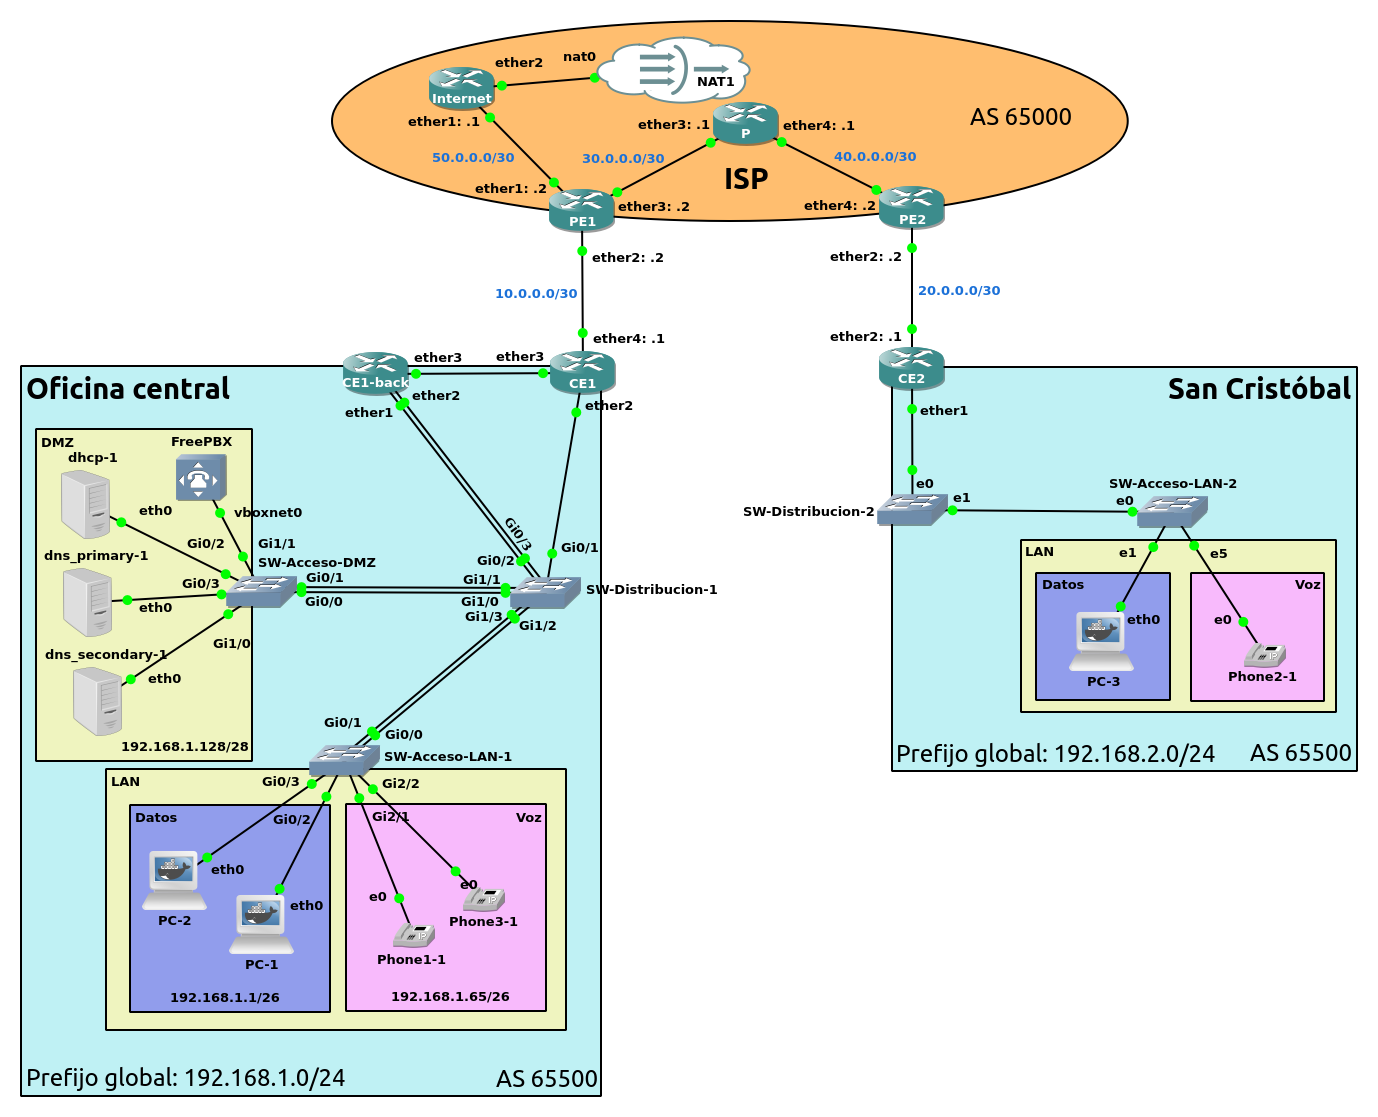
\includegraphics[width=0.9\textwidth]{images/simulacion_entera.png}
	\caption{Simulación de la red completa}
	\label{fig:simulation_office_sancristobal}
\end{figure}

Para la red ISP se ha tomado como referencia la topología L3 MPLS VPN del Trabajo de Fin de Grado de D. Carpio Ortiz
\cite{carpio2023tfg}, adaptándola a los requisitos de la simulación. Se han empleado cuatro routers MikroTik (PE1, PE2, P y un router conectado a una Cloud de GNS3), configurados de forma similar a lo descrito en la sección \ref{sec:simulacion_red_isp}. Además, se ha seguido el esquema de direccionamiento de la Tabla~\ref{tab:tabla_direccionamiento_red_completa} para asignar la red MPLS.

\begin{table}[htb]
	\centering
	\begin{subtable}[b]{0.475\textwidth}
		\centering
		\begin{tabular}{|l|l|l|}
			\hline
			\textbf{Router} & \textbf{Interfaz} & \textbf{Dirección IP} \\ \hline
			CE1             & Lo0               & 192.170.0.1/32        \\ \cline{2-3}
			                & ether1            & 10.0.0.1/30           \\ \cline{2-3}
			                & ether2            & 192.168.1.1/30        \\ \cline{2-3}
			                & ether3            & 10.0.0.14/30          \\ \hline
			PE1             & Lo0               & 192.170.0.2/32        \\ \cline{2-3}
			                & ether1            & 10.0.0.2/30           \\ \cline{2-3}
			                & ether2            & 30.0.0.2/30           \\ \cline{2-3}
			                & ether3            & 50.0.0.1/30           \\ \hline
			P               & Lo0               & 192.170.0.3/32        \\ \cline{2-3}
			                & ether1            & 30.0.0.1/30           \\ \cline{2-3}
			                & ether2            & 40.0.0.1/30           \\ \hline
		\end{tabular}
	\end{subtable}
	\hfill
	\begin{subtable}[b]{0.475\textwidth}
		\centering
		\begin{tabular}{|l|l|l|}
			\hline
			\textbf{Router} & \textbf{Interfaz} & \textbf{Dirección IP} \\ \hline
			PE2             & Lo0               & 192.170.0.4/32        \\ \cline{2-3}
			                & ether1            & 40.0.0.2/30           \\ \cline{2-3}
			                & ether2            & 20.0.0.2/30           \\ \hline
			CE2             & Lo0               & 192.170.0.5/32        \\ \cline{2-3}
			                & ether1            & 20.0.0.1/30           \\ \cline{2-3}
			                & ether2            & 192.168.2.1/30        \\ \hline
			Internet        & Lo0               & 192.170.0.1/32        \\ \cline{2-3}
			                & ether1            & 50.0.0.2/30           \\ \cline{2-3}
			                & ether2            & DHCP                  \\ \hline
		\end{tabular}
	\end{subtable}
	\caption{Esquema de direccionamiento para la red MPLS}
	\label{tab:tabla_direccionamiento_red_completa}
\end{table}

\vspace{0.5cm}
Para completar la simulación, se ha centralizado el acceso a Internet a través de la Oficina Central. De este modo,
todo el tráfico externo generado por los hosts de las sedes remotas (por ejemplo, San Cristóbal) no se dirige directamente fuera de su propia sede, sino que primero es redirigido a la Oficina Central. Allí, el router CE1 actúa como puerta de enlace principal, aplicando NAT al tráfico saliente. La configuración correspondiente en el router CE1 es la siguiente:

\begin{lstlisting}[language=RouterOS]
[admin@CE1] > /ip firewall nat add action=masquerade chain=srcnat dst-address=!192.168.0.0/16 out-interface=ether4
\end{lstlisting}

Esta regla de NAT se aplica a todo el tráfico que sale por la interfaz \texttt{ether4} (que está conectada a la red ISP) y que no tiene como destino una dirección de la red interna (192.168.0.0/16). Esto asegura que todo el tráfico de salida a Internet desde las sedes remotas sea enmascarado con la dirección IP pública del router CE1, permitiendo que los hosts de las sedes remotas puedan acceder a Internet a través de la Oficina Central. Además, se ha añadido una ruta estática para dirigir el tráfico hacia el router PE1 de la red ISP para que pueda salir a Internet.
\begin{lstlisting}[language=RouterOS]
[admin@CE1] > /ip route add gateway=10.0.0.2
\end{lstlisting}

En la Figura~\ref{traceroutePC3} se puede ver el resultado de un \texttt{traceroute} desde un PC en la sede San Cristóbal a un servidor de Google (8.8.8.8) donde se puede observar que el tráfico sale de la LAN de la sede remota, atraviesa el router CE2, luego viaja por la red backbone MPLS (VPN L3) hasta llegar al router CE1 en la Oficina Central, donde se reenvía al router PE1, que es el punto de salida hacia el ISP. Finalmente, el tráfico atraviesa el router de frontera a Internet y accede a la nube (Internet).

\begin{figure}[htb]
	\centering
	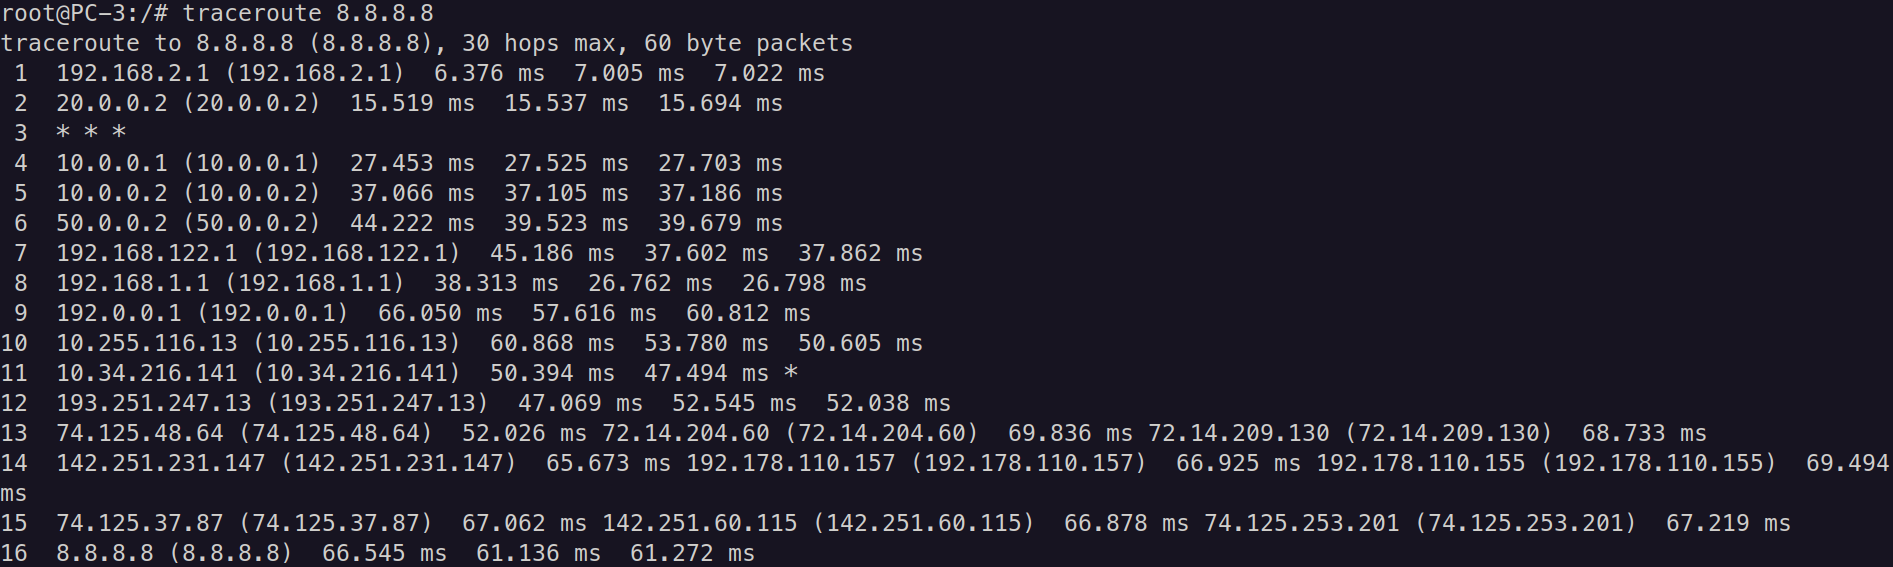
\includegraphics[width=0.95\textwidth]{images/traceroute_PC3_toInternet.png}
	\caption{Resultado de un traceroute desde un PC San Cristóbal a Internet}
	\label{traceroutePC3}
\end{figure}

Por otro lado, las sedes tienen direccionamiento IPv4 para simplificar la simulación ya que los routers MikroTik tienen algunas limitaciones con IPv6, como la falta de soporte para trabajar con MPLS. Por lo tanto, la Oficina Central tendrá una configuración similar a la que se realizó anteriormente, pero con direccionamiento IPv4 con un prefijo \texttt{192.168.1.0/24}. Para los servidores de red, se han creado contenedores Docker personalizados para el servicio DHCP y para el servicio DNS, con una configuración similar a la utilizada en la simulación de la Oficina Central, pero adaptada a direccionamiento IPv4. En los apéndices \ref{Apendice2:configuracion_dhcp_red_completa} y \ref{Apendice2:configuracion_dns_red_completa} se puede consultar la configuración detallada de cada uno de estos servicios. En cuanto a los switches de la Oficina Central, se ha utilizado los de la simulación de la Oficina Central y con la misma configuración.

\vspace{0.5cm}
En cuanto a la sede de San Cristóbal se ha realizado una configuración básica, donde se ha usado un router MikroTik identifiado como CE2 \ref{Apendice2:configuracion_ce2_san_cristobal} con un prefijo \texttt{192.168.2.0/24} y se ha usado switches ethernet de GNS3 para hacer una configuración sencilla de VLANs y conectividad. En la figura \ref{fig:switches_san_cristobal} se puede ver la configuración de los switches de la sede de San Cristóbal.

\begin{figure}[H]
	\centering
	\begin{subfigure}[b]{0.49\textwidth}
		\centering
		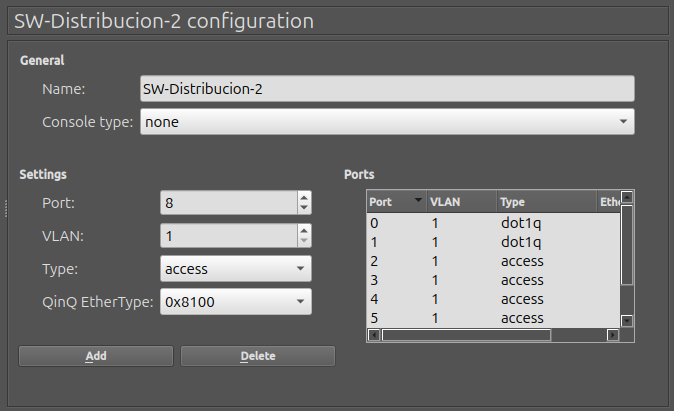
\includegraphics[width=\textwidth]{images/SanCristobal_SW-Distribucion_configuration.png}
		\caption{Switch de distribución de San Cristóbal}
		\label{subfig:switches_san_cristobal_1}
	\end{subfigure}
	\hfill
	\begin{subfigure}[b]{0.49\textwidth}
		\centering
		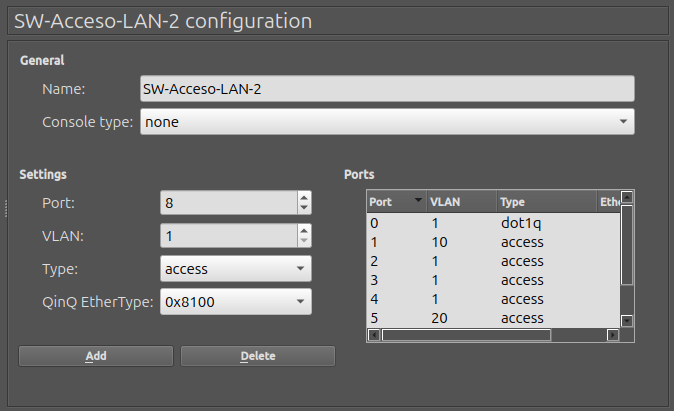
\includegraphics[width=\textwidth]{images/SanCristobal_SW-Acceso_configuration.png}
		\caption{Switch de acceso de San Cristóbal}
		\label{subfig:switches_san_cristobal_2}
	\end{subfigure}
	\caption{Configuración de los switches de la sede de San Cristóbal}
	\label{fig:switches_san_cristobal}
\end{figure}

En esta sede se ha configurado en el propio router CE2 un servidor DHCP (para simplificar la configuracion), que asigna las direcciones IP a los dispositivos de la red. Para ello, se ha creado un pool de direcciones IP para cada VLAN y se ha configurado el servidor para que asigne direcciones IP dentro de estos pools. Además, se ha configurado el gateway para cada VLAN.
\begin{lstlisting}[language=RouterOS]
# Pool de direcciones DHCP
/ip pool add name=pool_datos ranges=192.168.2.2-192.168.2.30
/ip pool add name=pool_voz ranges=192.168.2.34-192.168.2.62

# Servidor DHCP para VLAN 10 (Datos)
/ip dhcp-server add name=dhcp_datos interface=vlan10-datos address-pool=pool_datos disabled=no
/ip dhcp-server network add address=192.168.2.0/26 gateway=192.168.2.1

# Servidor DHCP para VLAN 20 (Voz)
/ip dhcp-server add name=dhcp_voz interface=vlan20-voz address-pool=pool_voz disabled=no
/ip dhcp-server network add address=192.168.2.32/26 gateway=192.168.2.33
\end{lstlisting}

Por último, para la conectividad de los dispositivos finales, se han creado contenedores Docker personalizados que actúan como PCs de prueba, parecidos a los utilizados en la Oficina Central pero para funcionar en IPv4. Además, como softphone se ha usado una máquina virtual ligera que viene instalada con algunas aplicaciones VoIP, obtenida de un tutorial de \texttt{Youtube} de C. E. Carrillo Arellano \cite{youtube_carlos_carrillo}. En esta máquina virtual viene instalado algunos softphones como \texttt{Zoiper} y \texttt{Microsip} y se ha configurado para que se pueda usar en la VLAN de voz. Para la centralita de telefonía IP se ha instalado \texttt{FreePBX} en una máquina virtual en \texttt{VirtualBox} y se ha configurado con una IP estática \texttt{192.168.1.135} y se ha conectado en la DMZ de la Oficina Central. Para simplificar la configuración, esta centralita se ha configurado para que pueda gestionar las llamadas entre los teléfonos IP de la Oficina Central y se han creado dos extensiones para comprobar la comunicación entre
los teléfonos IP de esta sede. En la Figura~\ref{fig:test_voip_ipv4} se puede ver la comprobación de la VoIP, donde se puede ver que se ha realizado una llamada entre dos teléfonos IP y se ha establecido la comunicación correctamente.

\begin{figure}[H]
	\centering
	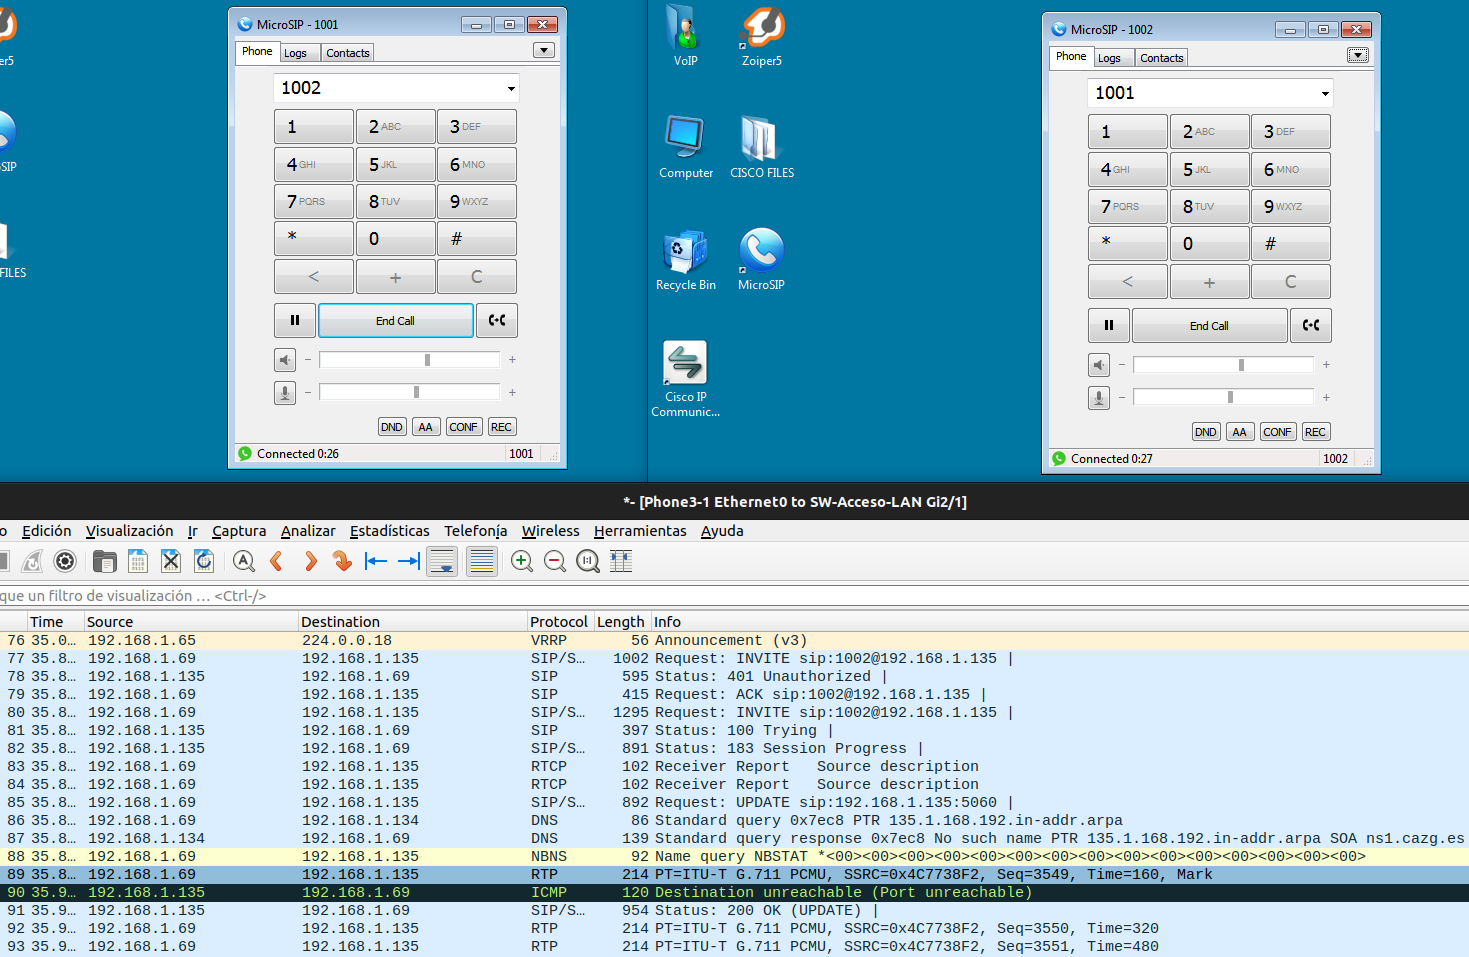
\includegraphics[width=0.8\textwidth]{images/test_voip_ipv4.png}
	\caption{Comprobación de la VoIP sobre IPv4}
	\label{fig:test_voip_ipv4}
\end{figure}

\section{Laboratorio}
En esta sección se describe la prueba que se realizó en el laboratorio efectuada para comprobar la comunicación entre dos teléfonos IP utilizando dispositivos físicos. Para ello, se emplearon un router \texttt{MikroTik RB2011UiAS-RM}, switches \texttt{TP-Link T2500G-10TS} y teléfonos IP \texttt{Grandstream GRP2601}. Los servicios de red DHCP y DNS se implementaron de forma simulada mediante GNS3 y se han usado los mismos contenedores que se han usado para las simulación de la red completa \ref{sec:simulacion_completa}. Estos contendores se estarán ejecutando en un ordenador físico (PC1) del laboratorio siguiendo el esquema de la Figura~\ref{fig:servicios_red_laboratorio}.

\begin{figure}[H]
	\centering
	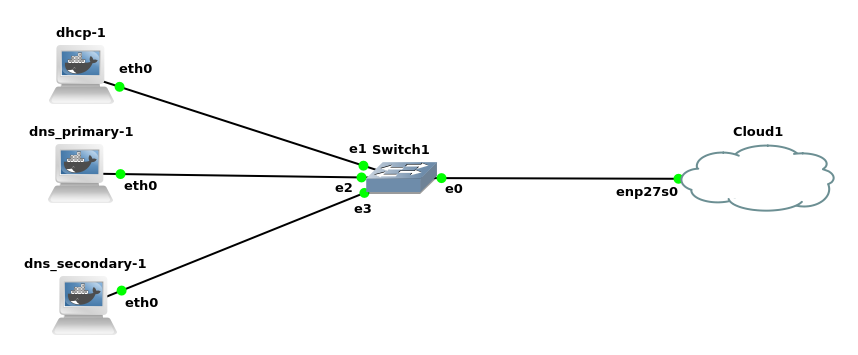
\includegraphics[width=0.75\textwidth]{images/servicios_red_laboratorio.png}
	\caption{Servicios de red utilizados en el laboratorio}
	\label{fig:servicios_red_laboratorio}
\end{figure}

Además, se ha usado otro ordenador físico (PC2) para operar como la centralita FreePBX y se ha ejecutado un contenedor Docker con
la imagen de FreePBX, y en este PC se ha configurado con una IP estática \texttt{192.168.1.135}. El docker-compose para la centralita
que se ha usado se encuentra en el apéndice \ref{Apendice2:docker_compose_freepbx}. En la Figura~\ref{fig:interconexion_red_laboratorio} se muestra
la interconexión que se ha realizado en el laboratorio.
\begin{figure}[H]
	\centering
	\begin{subfigure}[b]{0.59\textwidth}
		\centering
		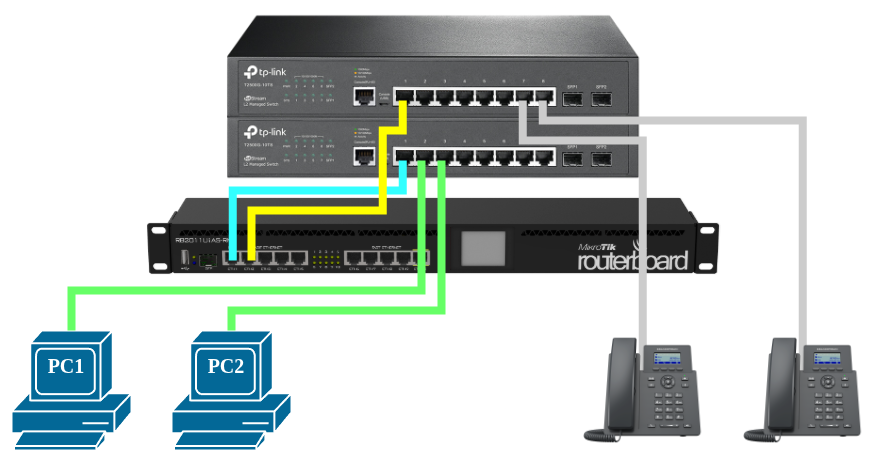
\includegraphics[width=\textwidth]{images/interconexion_red_laboratorio.png}
		\caption{Interconexión de los dispositivos}
		\label{fig:interconexion_red}
	\end{subfigure}
	\hfill
	\begin{subfigure}[b]{0.39\textwidth}
		\centering
		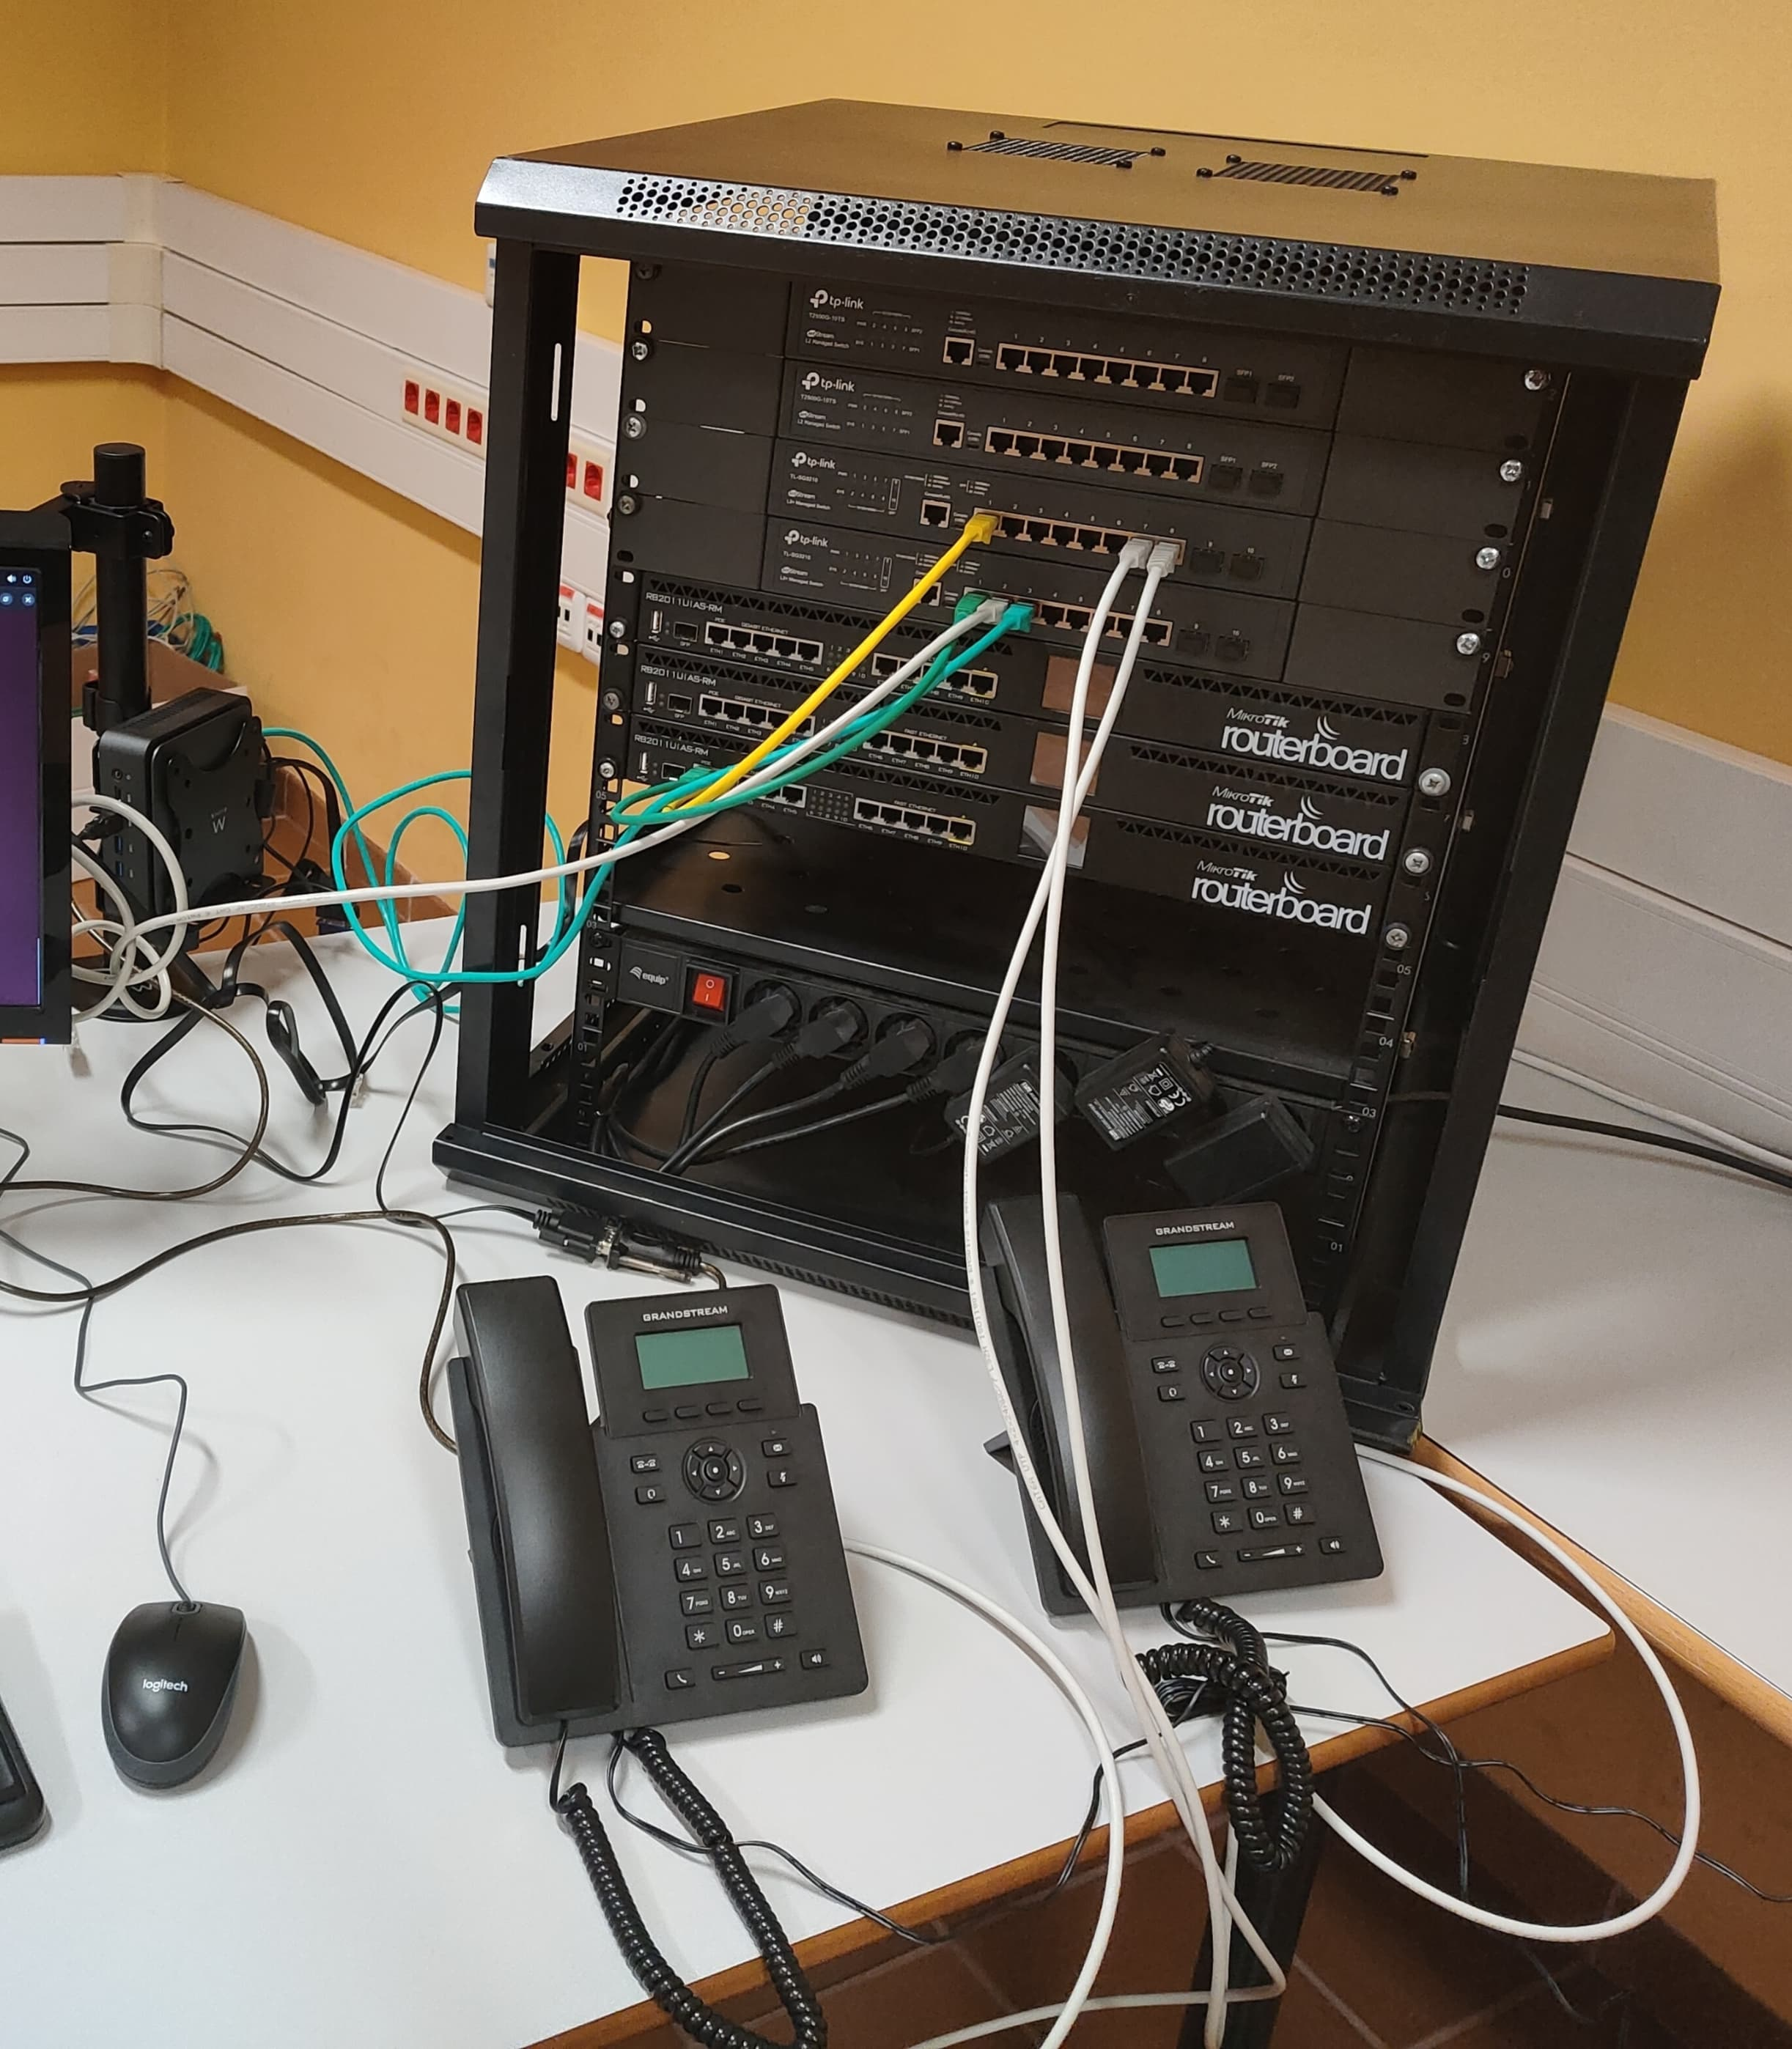
\includegraphics[width=\textwidth]{images/laboratorio.jpeg}
		\caption{Dispositivos físicos del laboratorio}
		\label{fig:laboratorio}
	\end{subfigure}
	\caption{Interconexión de red y dispositivos físicos utilizados en el laboratorio}
	\label{fig:interconexion_red_laboratorio}
\end{figure}

Por otro lado, en la centralita FreePBX se han creado dos extensiones, 1001 y 1002, destinadas al uso con teléfonos
IP, como se muestra en la Figura~\ref{fig:extensiones_telefonoIP}. Estas extensiones permiten realizar y recibir
llamadas dentro de la red local del sistema de telefonía.

\begin{figure}[H]
	\centering
	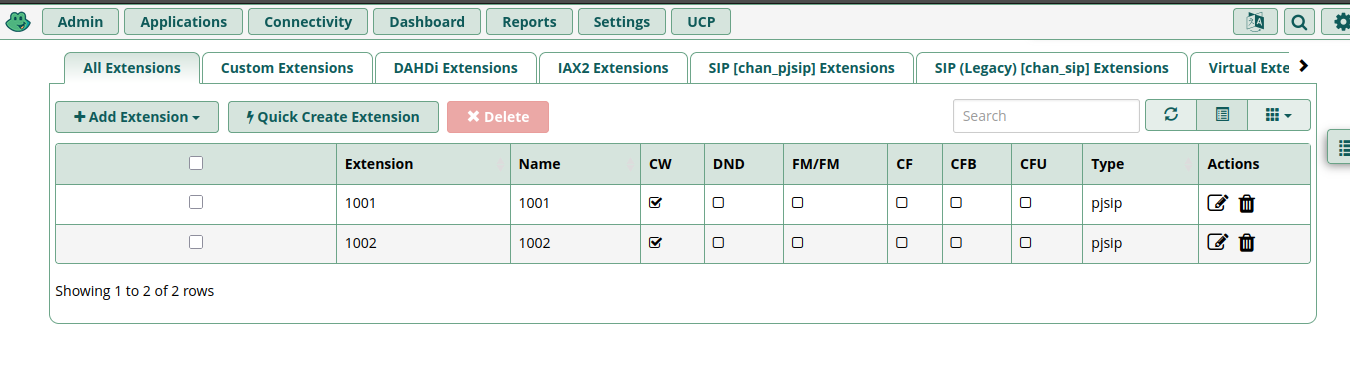
\includegraphics[width=1\textwidth]{images/extensiones_telefonoIP.png}
	\caption{Extensiones configuradas en la centralita FreePBX}
	\label{fig:extensiones_telefonoIP}
\end{figure}

Para cada una de estas extensiones se ha configurado un buzón de voz, permitiendo que los usuarios dejen mensajes
cuando no se puede atender una llamada. Esta funcionalidad resulta especialmente útil en entornos donde no siempre
es posible responder inmediatamente. En la Figura~\ref{fig:configuracion_buzon_voz} se muestra un ejemplo de esta
configuración, correspondiente a la extensión 1001. Entre las opciones disponibles se encuentran la definición de
la contraseña del buzón, el envío de mensajes por correo electrónico, y la posibilidad de reproducir el
identificador de llamada (CID) y los datos del mensaje (fecha y hora).

\begin{figure}[H]
	\centering
	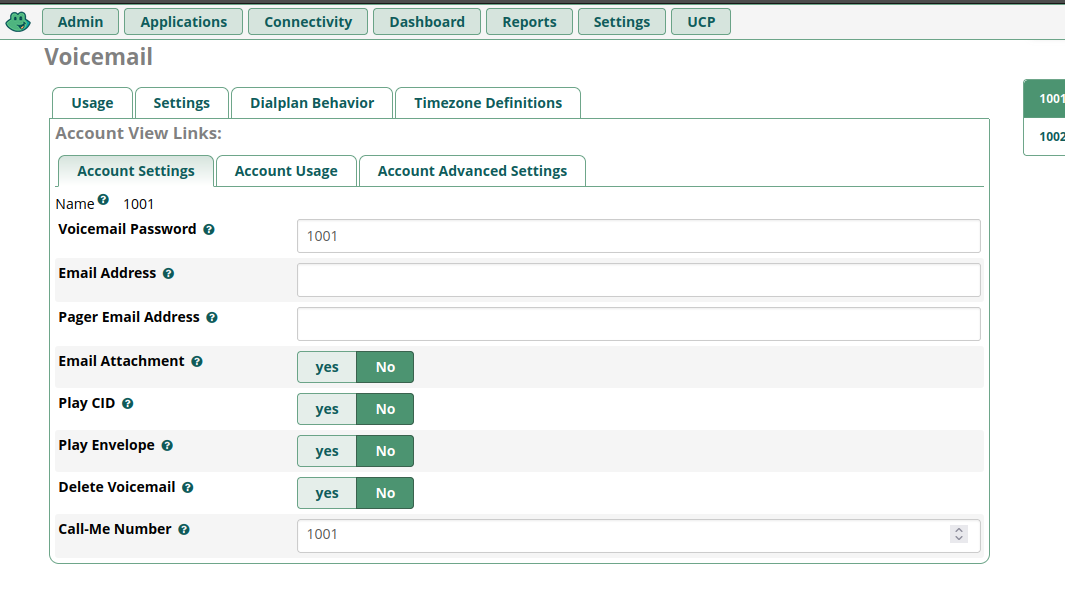
\includegraphics[width=0.8\textwidth]{images/configuracion_buzon_voz.png}
	\caption{Configuración del buzón de voz para la extensión 1001}
	\label{fig:configuracion_buzon_voz}
\end{figure}

Por último, los dispositivos conectados a la red obtienen sus direcciones IP mediante el protocolo DHCP,
el cual se encuentra ejecutándose en el ordenador físico (PC1) del laboratorio.
